\documentclass[11pt,a4paper]{amsart}

\usepackage{amsmath,amssymb,amsthm,mathtools}
\usepackage[T1]{fontenc}
\usepackage[utf8]{inputenc}
\usepackage{lmodern}
\usepackage{microtype}
\usepackage{graphicx}
\usepackage{hyperref}
\usepackage{orcidlink}
\usepackage{enumitem}
\usepackage[margin=1in]{geometry}
\raggedbottom

\theoremstyle{plain}
\newtheorem{theorem}{Theorem}[section]
\newtheorem{proposition}[theorem]{Proposition}
\newtheorem{lemma}[theorem]{Lemma}
\newtheorem{corollary}[theorem]{Corollary}

\theoremstyle{definition}
\newtheorem{definition}[theorem]{Definition}
\newtheorem{assumption}[theorem]{Assumption}

\theoremstyle{remark}
\newtheorem{remark}[theorem]{Remark}

\DeclareMathOperator{\Var}{Var}
\DeclareMathOperator{\Cov}{Cov}
\DeclareMathOperator{\tr}{tr}
\DeclareMathOperator{\rank}{rank}
\DeclareMathOperator{\diag}{diag}
\DeclareMathOperator{\spr}{spr}
\newcommand{\R}{\mathbb{R}}
\newcommand{\N}{\mathbb{N}}
\newcommand{\PP}{\mathbb{P}}
\newcommand{\QQ}{\mathbb{Q}}
\newcommand{\EE}{\mathbb{E}}
\newcommand{\one}{\mathbf{1}}
\newcommand{\dd}{\,d}
\newcommand{\toP}{\xrightarrow{\PP}}
\newcommand{\toD}{\xrightarrow{d}}
\newcommand{\cH}{\mathcal{H}}
\newcommand{\cF}{\mathcal{F}}
\newcommand{\cG}{\mathcal{G}}
\newcommand{\cE}{\mathcal{E}}

\begin{document}

\title[A Rough Theory of Markets]{%
A Rough Theory of Markets\\[0.3em]
{\small Latent Contagion, Market Phases,\\[0.15em]
and Market-Variance Risk}}
\author[J.~Vidal Llaurad\'o]{J.~Vidal Llaurad\'o\,\orcidlink{0009-0002-1918-5458}}
\thanks{DOI: \href{https://doi.org/10.2139/ssrn.6616121}{10.2139/ssrn.6616121}.}
\email{vidal.llaurado@gmail.com}
\subjclass[2020]{60G22, 62M15, 91G80, 62F12}
\keywords{rough volatility, latent contagion, Gaussian Volterra markets, market phases, Perron synchronization, market-variance risk, visible pricing and hedging}
\date{April 2026}

\begin{abstract}
Microscopic volatility can remain continuous while market-level observations become rough,
jump-like at coarse resolution, and only partially hedgeable.  This paper studies that separation
in an \(N\)-asset Gaussian Volterra market with directed latent-contagion kernels and aggregate
market-volatility functional \(M\).  Market-scale admissibility is selected by the projected
experiment, not imposed as a rough subclass.  An active off-diagonal channel is admissible exactly
when it remains source-screened visible, carries nonzero market loading, and admits a genuinely
shrinking projected local normalization; under the high-frequency market array this is equivalent to
\(H_{ij}<1/2\) together with source-screened visibility.

Within the admissible class, smooth directional contagion is locally degenerate at high frequency.
Rough channels are the stable observable high-frequency contagion phase.  If the market-dominant
admissible channels aggregate without leading-order cancellation, the aggregate market-volatility
exponent is the roughest active source-screened exponent and is strictly below one half.  The same
dominant edges define a screened synchronization matrix on the \(N\times N\) network.  Crossing its
Perron threshold aligns latent stress along a common mode and turns local rough propagation into
macroscopic amplification.  Under threshold-triggered activation, synchronized bursts whose widths
contract faster than observation resolution converge for coarse observers to a stochastic jump
limit, although the primitive market paths remain continuous.

The synchronized mode also carries the pricing and hedging obstruction.  For integrated market
variance \(Q_M=\int_0^T M(t)^2\,dt\), compression to any visible pricing summary leaves a
lower-bounded latent convexity gap, and visible hedges for variance-linked claims satisfy an
explicit lower bound on residual risk whenever the synchronized latent mode retains conditional
variance.  The reduction from Volterra primitives to these claims is derived from the canonical
Perron projection of the latent envelope and an aggregate sufficient-state sigma-field; no
pricing-side factor split is postulated.  Leading-order short-maturity skew statistics of the type
isolated in \cite{vidal2026latent} are visible \(\QQ\)-summaries, but they remain incomplete
relative to latent market-variance convexity.  The resulting phase classification connects
asymmetric latent contagion, roughness, Perron synchronization, coarse-observation jump limits, and
public compression of market-variance risk.
\end{abstract}

\maketitle

\section{Introduction}
Rough-volatility models give a tractable language for fractional memory and short-maturity scaling
\cite{gatheral2018volatility,livieri2018rough}.  They usually begin with a rough volatility law
and then study pricing, simulation, filtering, or calibration
\cite{bayer2016pricing,eleuch2019roughheston,abijaber2019affine}.  That route does not decide when
a market must become rough because its visible high-frequency experiment admits directed
latent-contagion channels.  The present construction starts from the directed market experiment.
Roughness is the consequence of source-screened local admissibility, not the primitive regularity
assumption.

The observable market object is the aggregate market-volatility functional \(M\).  The latent object
is an \(N\times N\) Gaussian Volterra system whose off-diagonal kernels transmit volatility from
source drivers to target assets.  A channel is economically active only when its market loading is
nonzero.  It is statistically admissible only when it remains visible after source screening and
admits a shrinking projected local normalization in the minimax experiment of
\cite{vidal2026econometric}.  Under the high-frequency market array, these requirements select
rough off-diagonal channels with \(H_{ij}<1/2\).  Smooth channels do not disappear from the
primitive model; they fail to generate a nondegenerate shrinking projected experiment.

This separates roughness from specification.  Section~\ref{sec:admissibility} characterizes the
projected-minimax admissible class before any aggregate roughness theorem is used.  Source-screened
visibility, nonzero market loading, and \(H_{ij}<1/2\) are necessary and sufficient for an active
off-diagonal channel to produce a finite nonzero projected local experiment.  The local information
geometry therefore selects the market-scale class rather than imposing roughness as a convenient
subclass.  The projected-score evidence in \cite{vidal2026econometric} supplies the
corresponding finite-panel diagnostic for realized-volatility data.

Three literatures determine the boundary of the construction.  Rough-volatility models supply the
Volterra scaling language, but in standard pricing applications the rough law is specified rather
than recovered from a market experiment \cite{gatheral2018volatility,bayer2016pricing,cont2024artefact}.
Network contagion and connectedness methods summarize spillovers, variance decompositions, and
crisis comovement, but they usually operate on visible dependence objects rather than on a
source-screened local likelihood geometry \cite{diebold2009spillovers,diebold2014connectedness,forbes2002interdependence}.
The latent-contagion observability strand separates source effects from target-only confounding and
identifies the projected local information geometry
\cite{vidal2026latent,vidal2026dynamic,vidal2026econometric}.  The present paper places these three
roles in one \(N\)-asset Volterra market: the Volterra kernels define the primitive channels, the
projected experiment selects the admissible active edges, and the market aggregation turns those
edges into roughness, synchronization, and public compression.

The comparison with the classic ``no contagion, only interdependence'' argument of
\cite{forbes2002interdependence} is at the level of the observed object.  Forbes and Rigobon ask
whether crisis comovement in returns exceeds visible interdependence after correcting for
heteroskedasticity.  Here the object is a directional latent-volatility channel that survives source
screening at the local scale.  A synchronized latent network can amplify market-wide stress while
remaining close to interdependence in reduced-form correlation measures.  Visible crisis
correlation alone does not certify contagion.  The theorem instead isolates latent directed channels
whose aggregate effects are roughness, Perron synchronization, and incomplete visible pricing and
hedging summaries.

The comparison with incomplete-information pricing is different.  The hidden object is the
synchronized volatility mode generated by the directed contagion network, rather than a private
signal or an exogenous equilibrium state.  Prices are treated as public compressions, not as noisy
measurements of an external factor.  Visible pricing summaries are incomplete because public
compression removes part of a latent rough mode that remains only partially screenable under
\(\QQ\).  The compression statements
below are instantiated for CoVaR-type tail summaries \cite{adrian2016covar}, SRISK-style shortfall
functionals \cite{brownlees2017srisk}, and Diebold--Y\i lmaz connectedness measures
\cite{diebold2009spillovers,diebold2014connectedness}.

The empirical layer is deliberately narrow.  Appendix~\ref{app:perron-validation} reports an
Oxford-Man Perron illustration with no unused-sample trading or theorem-validation status.  The
theoretical input comes from the projected observability results of \cite{vidal2026econometric}.  Admissibility fixes the active local experiment.  Roughness is the
resulting high-frequency phase.  The screened synchronization matrix then separates rough local
propagation from Perron synchronization.  Above the Perron threshold, the dominant rough edges align
latent stress along a common mode.  Under threshold-triggered activation, that mode can become
jump-like for coarse observers.  The same mode carries the market-variance convexity and hedge
shortfall left by visible compression.

The pricing statement stays at the compression level.  The threshold analysis in
\cite{vidal2026latent} isolates visible \(\QQ\)-side statistics, such as leading-order
short-maturity skew, that can fail to identify latent contagion even when the physical law remains
distinguishable.  The present paper extends that asymmetry to market scale.  Visible pricing
summaries may be well defined and fully observable while latent market-variance convexity and
hedging exposure remain outside the visible sigma-field.

The results follow the objects they identify.  Section~\ref{sec:admissibility} characterizes the
active off-diagonal channels that are projected-minimax admissible.  Within that class,
Theorem~\ref{thm:market-roughness} proves that market-dominant admissible asymmetry forces
\(H_M<1/2\).  Theorem~\ref{thm:synchronization} separates local roughness from systemic
synchronization through the Perron threshold of the screened synchronization matrix.
Theorem~\ref{thm:jump-appearance} and Corollary~\ref{cor:threshold-jumps} characterize the
jump-like limit produced by synchronized rough amplification under activated concentration.
Theorem~\ref{thm:sufficient-state-aggregate} derives the aggregate sufficient-state sigma-field
from primitive coupling, canonical Perron projection, and off-Perron screening.
Proposition~\ref{prop:q-decomposition} extracts the centered synchronized factor content of
integrated market variance.  Theorem~\ref{thm:compression} then proves the visible-price and
visible-hedge compression bounds.  Theorem~\ref{thm:market-phases} collects these statements into a
market-scale classification of contagion phases.

The phase classification is deliberately narrow.  A \emph{smooth-degenerate} regime has only
smooth active off-diagonal channels and no nondegenerate shrinking projected local contagion
experiment.  A \emph{rough-observable} regime has admissible dominant asymmetry and rough aggregate
volatility but no synchronized amplification.  A \emph{rough-synchronized} regime crosses the
screened Perron threshold and aligns stress along a common latent mode.  An \emph{activated
synchronized} regime adds threshold-triggered concentration of that mode, so continuous latent
synchronization becomes jump-like at coarse observation scales.  These phases classify directional
contagion, not all market dislocations.  They do not rule out rough idiosyncratic diagonal
channels.  What the smooth-degenerate phase excludes is a nondegenerate off-diagonal projected
contagion experiment.

The remaining sections follow this construction.  Section~\ref{sec:model} introduces the
\(N\)-asset directed Volterra market.  Section~\ref{sec:admissibility} derives local observability
and admissibility at market scale, and Section~\ref{sec:roughness} proves the aggregate roughness
law.  Section~\ref{sec:sync} studies the screened synchronization matrix and its Perron threshold.
Section~\ref{sec:jumps} derives the endogenous jump appearance at coarse observation scales.
Section~\ref{sec:implications} develops the pricing, convexity, and hedging compression results,
and Section~\ref{sec:conclusion} concludes.
\section[\texorpdfstring{An N-Asset Directed Volterra Market}{An N-Asset Directed Volterra Market}]{\texorpdfstring{An \(N\)-Asset Directed Volterra Market}{An N-Asset Directed Volterra Market}}\label{sec:model}

The primitive object is a directed Volterra volatility network.  Its off-diagonal kernels are the
candidate contagion channels; market aggregation will later decide which of them survive the
projected local experiment.

Let \(N\ge2\) be fixed and let \(W=(W^1,\dots,W^N)\) be an \(N\)-dimensional Brownian motion with
independent coordinates on a filtered probability space
\((\Omega,\cF,(\cF_t)_{t\ge0},\PP)\).  Asset \(i\) carries latent volatility channel
\[
        V_i(t)
        =
        \mu_i(t)
        +
        \sum_{j=1}^N
        \int_0^t
        K_{ij}(t,s)\,\dd W^j_s,
        \qquad
        1\le i\le N,
        \quad
        0\le t\le T.
\]
The kernel \(K_{ij}\) encodes the influence of latent driver \(j\) on asset \(i\).  The diagonal
terms \(K_{ii}\) are idiosyncratic; the off-diagonal terms \(K_{ij}\), \(i\neq j\), are directed
latent contagion channels.

\begin{assumption}[Directed Volterra regularity]\label{ass:volterra-market}
For every \(i,j\) there exist exponent \(H_{ij}\in(0,1)\), amplitude \(\beta_{ij}\in\R\), and a
continuous function \(a_{ij}\colon [0,T]^2\to\R\) such that for \(0\le s<t\le T\),
\[
        K_{ij}(t,s)
        =
        \beta_{ij}\,a_{ij}(t,s)\,(t-s)^{H_{ij}-1/2}.
\]
Moreover \(a_{ij}(t,t)>0\) whenever \(\beta_{ij}\neq0\), and the drift \(t\mapsto \mu_i(t)\) is
deterministic and continuous.
\end{assumption}

\begin{definition}[Aggregate market volatility]
Fix deterministic weights \(w=(w_1,\dots,w_N)\in(0,\infty)^N\).  The aggregate market-volatility
process is
\[
        M(t)
        =
        \sum_{i=1}^N w_i V_i(t).
\]
Its effective short-scale exponent \(H_M\) is defined by the requirement that for every interior
time \(t\in(0,T)\),
\[
        \Var\bigl(M(t+h)-M(t)\bigr)
        =
        c_M(t)\,h^{2H_M}
        +o(h^{2H_M})
        \qquad
        \text{as } h\downarrow0,
\]
for some deterministic \(c_M(t)>0\).
\end{definition}

\section{Local observability and admissibility at market scale}\label{sec:admissibility}

Admissibility is selected before aggregate roughness is proved.  The projected experiment fixes the
local scale of an active edge; the shrinking-scale condition then separates rough source-screened
channels from smooth or only \(O(1)\)-visible channels.

\begin{assumption}[High-frequency market resolution]\label{ass:market-resolution}
There exists a triangular array of local market blocks indexed by \(n\), with block width
\(h_n\downarrow0\) and block count \(N_n\uparrow\infty\), such that
\[
        N_n h_n \to \tau\in(0,\infty).
\]
For each active edge, \(I_{ij,n}^{\mathrm{eff}}\) denotes the effective information count in the
projected local experiment.  In an independent-block idealization
\(I_{ij,n}^{\mathrm{eff}}=N_n\).  In an overlapping-block implementation it is the corresponding
HAC-effective count, denoted \(N_{ij,n}^{\mathrm{HAC}}\).  The market-admissibility statements below
use \(I_{ij,n}^{\mathrm{eff}}h_n\) in place of a raw grid count and assume, for active visible
edges, that it stays bounded away from zero and infinity; write
\[
        I_{ij,n}^{\mathrm{eff}}h_n\to\tau_{ij}\in(0,\infty)
\]
when a limit is needed.
\end{assumption}

\begin{proposition}[Projected local scale from the market experiment]\label{prop:projected-scale}
Fix an edge \((i,j)\) with nonzero market loading, \(w_i\beta_{ij}\neq0\).  Suppose that
along the high-frequency array of Assumption~\ref{ass:market-resolution}, the source-screened
projected experiment for that edge admits blockwise score contributions \(S_{ij,\ell,n}\),
\(1\le \ell\le N_n\), such that under the null
\[
        \EE[S_{ij,\ell,n}] = 0,
        \qquad
        \Var(S_{ij,\ell,n}) = \kappa_{ij} h_n^{2H_{ij}} + o(h_n^{2H_{ij}})
\]
for some \(\kappa_{ij}>0\), and
\[
        \Var\!\left(\sum_{\ell=1}^{N_n} S_{ij,\ell,n}\right)
        =
        I_{ij,n}^{\mathrm{eff}}\kappa_{ij} h_n^{2H_{ij}}
        + o(I_{ij,n}^{\mathrm{eff}} h_n^{2H_{ij}}).
\]
Writing \(S_{ij,n}:=\sum_{\ell=1}^{N_n} S_{ij,\ell,n}\), assume moreover that for every shrinking
perturbation sequence \(\delta_n\to0\), the projected log-likelihood ratio admits the local
quadratic expansion
\[
        \log\frac{\dd \PP_{ij,n}^{(\delta_n)}}{\dd \PP_{ij,n}^{(0)}}
        =
        \delta_n S_{ij,n}
        -
        \frac12 \delta_n^2 \mathcal I_{ij,n}
        +
        o_{\PP}(1),
\]
with
\[
        \mathcal I_{ij,n}
        =
        I_{ij,n}^{\mathrm{eff}}\kappa_{ij} h_n^{2H_{ij}}
        + o(I_{ij,n}^{\mathrm{eff}}h_n^{2H_{ij}}).
\]
Then a local perturbation of amplitude \(\delta_n\) remains in the finite local quadratic
regime if and only if
\[
        \delta_n \sqrt{I_{ij,n}^{\mathrm{eff}}} h_n^{H_{ij}} = O(1).
\]
It is nondegenerate on a local sequence when this product is bounded away from zero and infinity.
Consequently the unique local normalization, up to constant multiples, that produces a finite
nonzero local experiment is
\[
        \theta_{ij,n}
        =
        (I_{ij,n}^{\mathrm{eff}})^{-1/2}h_n^{-H_{ij}}.
\]
\end{proposition}

\begin{proof}
Under the stated variance expansion, the aggregated projected score \(S_{ij,n}\) has standard
deviation
\[
        \sqrt{\Var(S_{ij,n})}
        =
        \sqrt{\kappa_{ij}}\,\sqrt{I_{ij,n}^{\mathrm{eff}}}h_n^{H_{ij}}\,(1+o(1)).
\]
Likewise,
\[
        \delta_n^2 \mathcal I_{ij,n}
        =
        \kappa_{ij}\bigl(\delta_n \sqrt{I_{ij,n}^{\mathrm{eff}}} h_n^{H_{ij}}\bigr)^2(1+o(1)).
\]
Set
\[
        \ell_n:=\delta_n \sqrt{I_{ij,n}^{\mathrm{eff}}} h_n^{H_{ij}}.
\]
The linear score term has stochastic size \(O_{\PP}(|\ell_n|)\), and the quadratic information
term has deterministic size \(O(\ell_n^2)\).  If \(\ell_n\to0\), both leading terms vanish and the
perturbation is asymptotically negligible.  If \(|\ell_n|\to\infty\), the quadratic term leaves
the finite local regime.  Finite nonzero local alternatives are obtained by keeping \(\ell_n\)
bounded and non-vanishing along the local sequence under consideration.  This fixes the local scale,
up to constant multiples, as
\[
        \theta_{ij,n}=(I_{ij,n}^{\mathrm{eff}})^{-1/2}h_n^{-H_{ij}}.
\]
\end{proof}

\begin{remark}[Imported input and market-level step]
The imported object from \cite{vidal2026econometric} is the source-screened projected experiment:
visible edges have strictly positive local information and satisfy the local quadratic expansion
used above.  Proposition~\ref{prop:projected-scale} performs the market-level step.  Once the
projected experiment is placed on a high-frequency market array, the local normalization is not a
chosen scale; it is the unique finite nonzero scale of the local log-likelihood.
\end{remark}

\begin{proposition}[Pairwise projected import is dimension-honest]\label{prop:pairwise-import}
Fix an ordered pair \((i,j)\).  The admissibility analysis in the present section uses from
\cite{vidal2026econometric} only the pairwise source-screened projected experiment attached to that
pair: source-screened visibility, a strictly positive projected information lower bound when the
channel is visible, and the corresponding local quadratic expansion on the high-frequency array.
Conditional on that pairwise input, Proposition~\ref{prop:projected-scale},
Lemma~\ref{lem:smooth-failure}, Definition~\ref{def:market-admissibility}, and
Proposition~\ref{prop:admissibility-characterization} are dimension-agnostic.  In particular, the
admissibility characterization does not rely on any bivariate ambient market restriction.
\end{proposition}

\begin{proof}
Every step in the admissibility block fixes one ordered pair \((i,j)\) and then uses only the
projected score variance, the projected information lower bound, and the projected local
normalization for that pair.  The ambient dimension \(N\) enters only through the choice of the
pair and the market-loading coefficient \(w_i\beta_{ij}\).  No argument reduces the full market to
a two-asset system.
\end{proof}

\begin{lemma}[Observability failure for smooth channels]\label{lem:smooth-failure}
Fix an off-diagonal edge \((i,j)\) with \(i\neq j\) and nonzero market loading
\(w_i\beta_{ij}\neq0\), and assume the blockwise score and local quadratic expansion hypotheses of
Proposition~\ref{prop:projected-scale}.  If \(H_{ij}\ge \tfrac12\), then for every shrinking
perturbation sequence \(\delta_n\to0\),
\[
        \delta_n S_{ij,n}\toP0
\]
and
\[
        \delta_n^2 \mathcal I_{ij,n}\to0.
\]
Consequently the projected local log-likelihood shift vanishes along every shrinking alternative, so
the edge does not generate a nondegenerate projected local experiment at high frequency.
\end{lemma}

\begin{proof}
Proposition~\ref{prop:projected-scale} gives
\[
        \sqrt{\Var(S_{ij,n})}
        =
        \sqrt{\kappa_{ij}}\,\sqrt{I_{ij,n}^{\mathrm{eff}}}h_n^{H_{ij}}(1+o(1))
        =
        \sqrt{\kappa_{ij}}\,(I_{ij,n}^{\mathrm{eff}} h_n)^{1/2}h_n^{H_{ij}-1/2}(1+o(1)).
\]
Because \(I_{ij,n}^{\mathrm{eff}} h_n\to\tau_{ij}\in(0,\infty)\), the factor
\((I_{ij,n}^{\mathrm{eff}} h_n)^{1/2}\) stays bounded away from
zero and infinity.  If \(H_{ij}>\tfrac12\), then \(h_n^{H_{ij}-1/2}\to0\), so
\[
        \sqrt{\Var(S_{ij,n})}\to0.
\]
If \(H_{ij}=\tfrac12\), then \(\sqrt{\Var(S_{ij,n})}\to \sqrt{\kappa_{ij}\tau}\in(0,\infty)\).
Therefore in either case
\[
        \delta_n\sqrt{\Var(S_{ij,n})}\to0
\]
for every sequence \(\delta_n\to0\).  Chebyshev's inequality then yields
\[
        \delta_n S_{ij,n}\toP0.
\]
Moreover,
\[
        \mathcal I_{ij,n}
        =
        \kappa_{ij}(I_{ij,n}^{\mathrm{eff}} h_n)h_n^{2H_{ij}-1}(1+o(1)).
\]
If \(H_{ij}>\tfrac12\), then \(\mathcal I_{ij,n}\to0\).  If \(H_{ij}=\tfrac12\), then
\(\mathcal I_{ij,n}\to\kappa_{ij}\tau_{ij}\in(0,\infty)\).  Therefore in either case
\[
        \delta_n^2 \mathcal I_{ij,n}\to0.
\]
The local quadratic expansion in Proposition~\ref{prop:projected-scale} now yields
\[
        \log\frac{\dd \PP_{ij,n}^{(\delta_n)}}{\dd \PP_{ij,n}^{(0)}}
        =
        o_{\PP}(1),
\]
so both the linear score term and the quadratic information term vanish along every shrinking
alternative.  This proves the degeneracy claim.
\end{proof}

\begin{definition}[Active and dominant edges]
The active edge set is
\[
        \cE_{\mathrm{act}}
        =
        \{(i,j): w_i\beta_{ij}\neq0\}.
\]
When \(\cE_{\mathrm{act}}\neq\varnothing\), its dominant exponent and dominant edge set are
\[
        H_*
        =
        \min_{(i,j)\in \cE_{\mathrm{act}}} H_{ij},
        \qquad
        \cE_*
        =
        \{(i,j)\in \cE_{\mathrm{act}}: H_{ij}=H_*\}.
\]
All subsequent uses of \(H_*\) occur under assumptions that make the active set nonempty.
\end{definition}

\begin{assumption}[Noncancelling aggregation]\label{ass:noncancel}
The active edge set is nonempty.  For every interior time \(t\in(0,T)\),
\[
        \sum_{j=1}^N
        \left(
        \sum_{i:\,(i,j)\in\cE_*}
        w_i\beta_{ij}a_{ij}(t,t)
        \right)^2
        >0.
\]
Equivalently, the dominant short-scale contributions do not cancel at leading order in the
variance of \(M(t+h)-M(t)\).
\end{assumption}

\begin{definition}[Projected-minimax admissibility]\label{def:market-admissibility}
An active off-diagonal edge \((i,j)\in\cE_{\mathrm{act}}\) with \(i\neq j\) is called
\emph{projected-minimax admissible} if it satisfies both conditions.
\begin{enumerate}[label=(\roman*)]
\item the corresponding source-to-target channel remains source-screened visible in the projected
information geometry of \cite{vidal2026econometric}, so its projected information lower bound is
strictly positive at the local scale;
\item along the high-frequency array of Assumption~\ref{ass:market-resolution}, the projected
normalization
\[
        \theta_{ij,n}
        =
        (I_{ij,n}^{\mathrm{eff}})^{-1/2}h_n^{-H_{ij}}
\]
identified in Proposition~\ref{prop:projected-scale} is a genuinely local scale, in the sense that
\(\theta_{ij,n}\to0\).
\end{enumerate}
The set of admissible edges is denoted \(\cE_{\mathrm{adm}}\).
\end{definition}

\subsection{Admissible market classes}

\noindent
Proposition~\ref{prop:admissibility-characterization} characterizes the admissible class inside the
projected experiment.  Its proof uses only Definition~\ref{def:market-admissibility},
Proposition~\ref{prop:projected-scale}, and Lemma~\ref{lem:smooth-failure}.  Later roughness,
synchronization, and pricing results depend on this class; they do not enter its definition.

\begin{proposition}[Characterization of projected-minimax admissibility]\label{prop:admissibility-characterization}
Assume Assumption~\ref{ass:market-resolution} and fix an active off-diagonal edge
\((i,j)\in\cE_{\mathrm{act}}\) with \(i\neq j\).  Suppose the projected experiment attached to that edge
inherits a strictly positive projected information lower bound whenever the channel is
source-screened visible, as in \cite{vidal2026econometric}, and satisfies the blockwise score and
local quadratic expansion hypotheses of Proposition~\ref{prop:projected-scale}.  Then the
following are equivalent:
\begin{enumerate}[label=(\roman*)]
\item \((i,j)\) is projected-minimax admissible.
\item The channel remains source-screened visible in the projected experiment and satisfies
\[
        H_{ij}<\frac12.
\]
\end{enumerate}
\end{proposition}

\begin{proof}
If \((i,j)\) is projected-minimax admissible, source-screened visibility is part~(i) of
Definition~\ref{def:market-admissibility}.  Proposition~\ref{prop:projected-scale} identifies
\(\theta_{ij,n}=(I_{ij,n}^{\mathrm{eff}})^{-1/2}h_n^{-H_{ij}}\) as the only candidate finite nonzero local
normalization.  Under Assumption~\ref{ass:market-resolution},
\[
        \theta_{ij,n}
        =
        (I_{ij,n}^{\mathrm{eff}}h_n)^{-1/2}h_n^{1/2-H_{ij}}.
\]
If \(H_{ij}=1/2\), this scale converges to \(\tau_{ij}^{-1/2}\); if \(H_{ij}>1/2\), it diverges.
It is therefore not a shrinking local scale.  Lemma~\ref{lem:smooth-failure} gives the equivalent
likelihood statement: every shrinking perturbation is asymptotically invisible in the projected
experiment.  Definition~\ref{def:market-admissibility}(ii) is violated, and hence \(H_{ij}<1/2\).

Conversely, suppose \((i,j)\) is source-screened visible and satisfies \(H_{ij}<1/2\).
Proposition~\ref{prop:projected-scale} identifies the unique finite nonzero local
normalization as
\[
        \theta_{ij,n}
        =
        (I_{ij,n}^{\mathrm{eff}})^{-1/2}h_n^{-H_{ij}}
        =
        (I_{ij,n}^{\mathrm{eff}} h_n)^{-1/2}h_n^{1/2-H_{ij}}.
\]
Since \(I_{ij,n}^{\mathrm{eff}} h_n\to\tau_{ij}\in(0,\infty)\) and \(H_{ij}<1/2\), one has
\(\theta_{ij,n}\to0\).  The
positive projected information lower bound makes this shrinking scale nondegenerate in the
projected experiment.  Together with source-screened visibility, this gives
Definition~\ref{def:market-admissibility}.
\end{proof}

\begin{corollary}[Non-vacuity of the admissible class]\label{cor:admissibility-nonvacuous}
Assume Assumption~\ref{ass:market-resolution}.  If there exists an off-diagonal edge
\((i,j)\in\cE_{\mathrm{act}}\) such that \(i\neq j\), the channel is source-screened visible in the
projected experiment with strictly positive projected information, the corresponding projected
experiment satisfies the blockwise score and local quadratic expansion hypotheses of
Proposition~\ref{prop:projected-scale}, and
\[
        H_{ij}<\frac12,
\]
then
\[
        \cE_{\mathrm{adm}}\neq\varnothing.
\]
In particular, the admissibility class is nonempty whenever the market contains at least
one economically active rough source-screened contagion channel.  If, in addition, the dominant
market-scale edges lie in that same class, Theorem~\ref{thm:market-roughness} applies nontrivially.
\end{corollary}

\begin{proof}
This is the implication \((ii)\Rightarrow(i)\) in
Proposition~\ref{prop:admissibility-characterization}, applied to the given off-diagonal edge.
\end{proof}

\begin{remark}[Which channels are excluded]\label{rem:excluded-admissibility}
The admissibility class excludes two economically distinct cases.
\begin{enumerate}[label=(\roman*)]
\item Smooth off-diagonal contagion channels with \(H_{ij}\ge\tfrac12\), because they generate
degenerate shrinking projected experiments.
\item Off-diagonal channels that are visible only at an \(O(1)\) scale, because they do not admit a genuinely
local projected normalization.
\end{enumerate}
A channel with zero market loading does not belong to the active market-edge set in the first
place, so it is screened out before admissibility is assessed.
\end{remark}

\begin{remark}[Economic content of the admissible class]
Proposition~\ref{prop:admissibility-characterization} and
Corollary~\ref{cor:admissibility-nonvacuous} make the admissible class non-vacuous.  The class is
not an exogenous rough subclass.  It consists of source-screened channels that are statistically
visible, economically active, and genuinely local at high frequency.  The projected-score evidence
in \cite{vidal2026econometric} documents rough visible edges of this form in realized-volatility
panels, so the admissible class has empirical content as well as formal content.
\end{remark}

\begin{remark}[What the admissibility condition means]
Definition~\ref{def:market-admissibility} imports the source-screened observability and minimax
results of \cite{vidal2026latent,vidal2026dynamic,vidal2026econometric} into the market model and
selects the directed channels that remain source-screened visible and admit a genuinely local
projected experiment.  The shrinking-scale condition is the link to the minimax theory.  An edge visible only
at an \(O(1)\) scale is not a latent high-frequency channel in the projected LAN sense.
\end{remark}

\begin{lemma}[Local projected admissibility forces roughness]\label{lem:admissibility-rough}
Assume Assumption~\ref{ass:market-resolution}.  If an active off-diagonal edge \((i,j)\) is
projected-minimax admissible, then
\[
        H_{ij}<\frac12.
\]
\end{lemma}

\begin{proof}
Projected-minimax admissibility requires the normalization
\[
        \theta_{ij,n}
        =
        (I_{ij,n}^{\mathrm{eff}})^{-1/2}h_n^{-H_{ij}}
        =
        (I_{ij,n}^{\mathrm{eff}} h_n)^{-1/2}h_n^{1/2-H_{ij}}
\]
to be genuinely local, hence \(\theta_{ij,n}\to0\).  Since
\(I_{ij,n}^{\mathrm{eff}}h_n\to\tau_{ij}\in(0,\infty)\), this is
possible only when \(1/2-H_{ij}>0\).  Therefore \(H_{ij}<1/2\).
\end{proof}


\begin{lemma}[Driverwise dominant short-scale expansion]\label{lem:driver-expansion}
Under Assumption~\ref{ass:volterra-market}, assume \(\cE_{\mathrm{act}}\neq\varnothing\), fix an
interior time \(t\in(0,T)\) and a driver \(j\in\{1,\dots,N\}\).  Define
\[
        G_{j,h,t}(s)
        :=
        \sum_{i=1}^N
        w_i\bigl[K_{ij}(t+h,s)-K_{ij}(t,s)\bigr].
\]
Then there exists a constant \(\kappa(H_*)>0\), depending only on \(H_*\), such that
\[
        \int_0^{t+h} G_{j,h,t}(s)^2\,\dd s
        =
        \kappa(H_*)
        \left(
        \sum_{i:\,(i,j)\in\cE_*}
        w_i\beta_{ij}a_{ij}(t,t)
        \right)^2
        h^{2H_*}
        +o(h^{2H_*})
\]
as \(h\downarrow0\).
\end{lemma}

\begin{proof}
For \(H\in(0,1)\), write
\[
        \Gamma_{H,t,h}(s)
        :=
        (t+h-s)^{H-1/2}\one_{\{s<t+h\}}
        -
        (t-s)^{H-1/2}\one_{\{s<t\}}.
\]
Assumption~\ref{ass:volterra-market} and continuity of \(a_{ij}\) imply the local expansion
\[
        K_{ij}(t+h,s)-K_{ij}(t,s)
        =
        \beta_{ij}a_{ij}(t,t)\Gamma_{H_{ij},t,h}(s)
        +
        r_{ij,h,t}(s),
\]
where \(\|r_{ij,h,t}\|_{L^2([0,t+h])}=o(h^{H_{ij}})\).  The Riemann--Liouville increment kernel
satisfies the short-scale expansion from Lemma~\ref{lem:RL-scaling}.  Edges with
\(w_i\beta_{ij}=0\) contribute no leading aggregate term, regardless of their exponent.  Active
edges outside \(\cE_*\) have exponent strictly larger than \(H_*\), hence contribute only
\(o(h^{H_*})\) in \(L^2\).  The edges in \(\cE_*\) share the same leading kernel
\(\Gamma_{H_*,t,h}\).  It follows, using the finiteness of the network, that
\[
        G_{j,h,t}(s)
        =
        \left(
        \sum_{i:\,(i,j)\in\cE_*}
        w_i\beta_{ij}a_{ij}(t,t)
        \right)\Gamma_{H_*,t,h}(s)
        +
        o_{L^2}(h^{H_*}).
\]
Denote the coefficient in parentheses by \(A_j(t)\).  Since
\(\|\Gamma_{H_*,t,h}\|_{L^2}=O(h^{H_*})\), Cauchy--Schwarz gives
\[
        \|G_{j,h,t}\|_2^2
        =
        A_j(t)^2\|\Gamma_{H_*,t,h}\|_2^2
        +
        o(h^{2H_*}).
\]
Lemma~\ref{lem:RL-scaling} then gives the claimed squared-norm expansion.
\end{proof}

\begin{proposition}[Leading-order aggregate variance expansion]\label{prop:aggregate-leading}
Under Assumptions~\ref{ass:volterra-market} and~\ref{ass:noncancel}, for every interior time
\(t\in(0,T)\),
\[
        \Var\bigl(M(t+h)-M(t)\bigr)
        =
        c_M(t)\,h^{2H_*}
        +o(h^{2H_*})
        \qquad
        \text{as } h\downarrow0,
\]
where the leading coefficient is
\[
        c_M(t)
        =
        \kappa(H_*)
        \sum_{j=1}^N
        \left(
        \sum_{i:\,(i,j)\in\cE_*}
        w_i\beta_{ij}a_{ij}(t,t)
        \right)^2
        >0.
\]
\end{proposition}

\begin{proof}
Write \(\Delta_h M(t)=M(t+h)-M(t)\).  Since each \(\mu_i\) is deterministic, it contributes no
variance.  By linearity and It\^o isometry,
\[
        \Var(\Delta_h M(t))
        =
        \sum_{j=1}^N
        \int_0^{t+h}
        \Biggl(
        \sum_{i=1}^N
        w_i\bigl[K_{ij}(t+h,s)-K_{ij}(t,s)\bigr]
        \Biggr)^2
        \dd s.
\]
Applying Lemma~\ref{lem:driver-expansion} to each driver \(j\) yields
\[
        \Var(\Delta_h M(t))
        =
        \kappa(H_*)
        \sum_{j=1}^N
        \left(
        \sum_{i:\,(i,j)\in\cE_*}
        w_i\beta_{ij}a_{ij}(t,t)
        \right)^2
        h^{2H_*}
        +
        o(h^{2H_*}).
\]
Assumption~\ref{ass:noncancel} makes the coefficient of \(h^{2H_*}\) strictly positive, which gives
the claimed expansion.
\end{proof}

\begin{corollary}[Aggregate exponent is the minimum active exponent]\label{cor:aggregate-min}
Under Assumptions~\ref{ass:volterra-market} and~\ref{ass:noncancel}, the aggregate market
volatility satisfies
\[
        H_M
        =
        H_*.
\]
\end{corollary}

\begin{proof}
Proposition~\ref{prop:aggregate-leading} identifies the leading variance order as
\(h^{2H_*}\) with strictly positive coefficient.  The definition of \(H_M\) therefore gives
\(H_M=H_*\).
\end{proof}

\section{Roughness necessity for market volatility}\label{sec:roughness}

The aggregate short-scale exponent is the minimum active edge exponent.  The admissibility
restriction now changes that algebraic fact into a roughness theorem.  If the market-dominant
directed edges are source-screened visible, economically active, and genuinely local at high
frequency, the aggregate exponent cannot remain smooth.

\begin{assumption}[Admissible dominant asymmetry]\label{ass:admissible-asymmetry}
The market has at least one projected-minimax admissible off-diagonal edge, that is,
\[
        \cE_{\mathrm{adm}}\neq\varnothing.
\]
Moreover every market-dominant active edge is an admissible off-diagonal edge.
\[
\cE_*
\subseteq
\cE_{\mathrm{adm}}.
\]
In particular, the dominant short-scale market asymmetry is carried by admissible contagion
channels rather than by diagonal or inadmissible edges.
\end{assumption}

\begin{theorem}[Market roughness necessity]\label{thm:market-roughness}
Assume Assumptions~\ref{ass:volterra-market}, \ref{ass:market-resolution}, \ref{ass:noncancel}, and
\ref{ass:admissible-asymmetry}.  Assume moreover that every edge in \(\cE_*\) satisfies the local
quadratic projected-experiment hypotheses of Proposition~\ref{prop:projected-scale}.  Write
\[
        H_{\mathrm{adm}}
        =
        \min_{(i,j)\in\cE_{\mathrm{adm}}} H_{ij}.
\]
Then the aggregate market volatility is necessarily rough.
\[
        H_M
        =
        H_{\mathrm{adm}}
        <
        \frac12.
\]
In particular, any market satisfying the observability/minimax admissibility condition
cannot have a smooth aggregate volatility law once its market-dominant contagion channels are
economically active, source-screened, and shrinking-scale.
\end{theorem}

\begin{proof}
By Assumption~\ref{ass:admissible-asymmetry}, every market-dominant edge belongs to
\(\cE_{\mathrm{adm}}\).  Lemma~\ref{lem:admissibility-rough} therefore proves that every edge in
\(\cE_*\) satisfies \(H_{ij}<1/2\).  Since \(H_*\) is the minimum exponent over \(\cE_*\), we have
\[
        H_*
        <
        \frac12.
\]
By Definition~\ref{def:market-admissibility}, admissible edges are active off-diagonal edges, so
\(\cE_{\mathrm{adm}}\subseteq\cE_{\mathrm{act}}\).  Hence \(H_{\mathrm{adm}}\ge H_*\).  The inclusion
\(\cE_*\subseteq\cE_{\mathrm{adm}}\) from Assumption~\ref{ass:admissible-asymmetry} gives the
reverse inequality, and therefore \(H_{\mathrm{adm}}=H_*\).  Corollary~\ref{cor:aggregate-min} then yields
\[
        H_M
        =
        H_*
        =
        H_{\mathrm{adm}}
        <
        \frac12,
\]
which proves the claim.
\end{proof}

\begin{corollary}[Recovery of the bivariate theory]\label{cor:bivariate-face}
In the case \(N=2\), Theorem~\ref{thm:market-roughness} reduces to the low-dimensional face of the
bivariate latent-contagion results.  A nondegenerate admissible channel \(1\to2\) or
\(2\to1\) forces the aggregate exponent to be the exponent of that active source-screened channel,
so the market-level roughness law collapses to the bivariate latent-contagion geometry studied in
\cite{vidal2026latent,vidal2026dynamic,vidal2026econometric}.
\end{corollary}

\begin{remark}[Necessity is relative to the admissibility class]
Theorem~\ref{thm:market-roughness} applies to markets whose active directional channels are
source-screened observable and informative for minimax discrimination.
Propositions~\ref{prop:admissibility-characterization} and~\ref{cor:admissibility-nonvacuous}
characterize that class rather than stipulate it.  Within the class, the admissibility criterion
forces roughness instead of treating it as an empirical coincidence or free regularity choice.
\end{remark}

\section{Systemic synchronization in the screened network}\label{sec:sync}

Roughness identifies the dominant market-scale edges.  Synchronization asks whether those edges
remain local spillovers or align into a common Perron mode.  The screened synchronization matrix is
the object that separates these two regimes.

Fix an interior time \(t_0\in(0,T)\).  The synchronization analysis is local around \(t_0\), just as
the roughness theorem is local in the short-scale limit.

\begin{definition}[Dominant signed edge matrix and screened synchronization matrix]
Let
\[
        \cE_M
        =
        \{(i,j)\in\cE_{\mathrm{adm}}: H_{ij}=H_M\}
\]
be the set of admissible market-scale edges.  For each \((i,j)\in\cE_M\), let
\(\pi_{ij}\in(0,\infty)\) denote its projected visibility weight, inherited from the
source-screened information geometry and normalized so that the matrix below is a dimensionless
one-step amplification operator for the local stress envelope.  The signed directed edge matrix is
\[
        B_{ij}
        =
        \beta_{ij}\,a_{ij}(t_0,t_0)\,\one_{\{(i,j)\in\cE_M\}},
        \qquad 1\le i,j\le N.
\]
The screened synchronization matrix is the nonnegative matrix \(A=(A_{ij})_{1\le i,j\le N}\) with
\[
        A_{ij}
        =
        |B_{ij}|\,\pi_{ij}.
\]
The matrix \(B\) keeps signs and governs signed aggregate contributions.  The matrix \(A\) forgets
signs and governs Perron synchronization.
\end{definition}

\begin{definition}[Screened contagion graph]
The \emph{screened contagion graph} is the directed graph \(G_M\) on vertices
\(\{1,\dots,N\}\) with an arrow \(j\to i\) whenever \(A_{ij}>0\).  It is called
\emph{strongly connected} if every ordered pair of vertices is linked by a directed path, and
\emph{aperiodic} if the greatest common divisor of its directed cycle lengths is one.
\end{definition}

\begin{definition}[Dominant rough stress envelope]
An \(H_M\)-scale stress envelope at time \(t_0\) is a vector \(x=(x_1,\dots,x_N)\in[0,\infty)^N\)
such that the dominant short-scale contribution to asset \(i\) takes the form
\[
        x_i (t-s)^{H_M-1/2}
\]
up to \(o((t-s)^{H_M-1/2})\) as \(s\uparrow t_0\).  The corresponding market-scale reduced
dynamics are governed by repeated action of the screened synchronization matrix \(A\).  The network
is said to be in the \emph{synchronized regime} when \(\spr(A)>1\).
\end{definition}

\begin{lemma}[Market-to-envelope reduction]\label{lem:dominant-envelope}
Let \(x_m\in[0,\infty)^N\) be the coefficient vector of the dominant \(H_M\)-scale contribution
generated by the market after \(m\) rounds of admissible contagion around \(t_0\).  Then one
further round of dominant contagion produces
\[
        x_{m+1}=A x_m + o(1)
\]
at the level of leading-order coefficients.
\end{lemma}

\begin{proof}
At time \(t_0\), the leading contribution of a dominant admissible edge \((i,j)\in\cE_M\) is
\[
        \beta_{ij}a_{ij}(t_0,t_0)(t-s)^{H_M-1/2}.
\]
Multiplying by the projected visibility weight \(\pi_{ij}\) and the incoming envelope coefficient
\(x_{m,j}\), then summing over dominant incoming edges, gives the next leading contribution for
asset \(i\),
\[
        \sum_{j=1}^N
        |B_{ij}|\,\pi_{ij}\,x_{m,j}.
\]
All non-dominant edges have exponent strictly larger than \(H_M\), hence contribute only lower
order terms in the short-scale expansion.  Therefore the dominant market coefficients are reduced,
at leading order, by the matrix \(A\), which yields \(x_{m+1}=Ax_m+o(1)\).
\end{proof}

\begin{proposition}[Finite-horizon reduction to the screened recursion]\label{prop:finite-horizon-reduction}
Fix \(M\in\N\).  For each short-scale parameter \(h\downarrow0\), let
\((x_0^{(h)},\dots,x_M^{(h)})\subset[0,\infty)^N\) satisfy
\[
        x_{m+1}^{(h)}=A x_m^{(h)}+r_m^{(h)},
        \qquad
        0\le m<M,
\]
with
\[
        x_0^{(h)}\to x_0
        \qquad\text{and}\qquad
        \max_{0\le m<M}\|r_m^{(h)}\|\to0
\]
for some \(x_0\in[0,\infty)^N\).  Then
\[
        \max_{0\le m\le M}\|x_m^{(h)}-A^m x_0\|\to0.
\]
In particular, on every fixed contagion depth, the actual market envelope and the exact screened
recursion have the same high-frequency limit.
\end{proposition}

\begin{proof}
Write
\[
        e_m^{(h)}:=x_m^{(h)}-A^m x_0.
\]
Then
\[
        e_{m+1}^{(h)}
        =
        A e_m^{(h)}+r_m^{(h)},
        \qquad
        0\le m<M,
\]
with \(e_0^{(h)}=x_0^{(h)}-x_0\to0\).  Iterating the recursion yields
\[
        e_m^{(h)}
        =
        A^m e_0^{(h)}
        +
        \sum_{\ell=0}^{m-1}A^{m-1-\ell}r_\ell^{(h)}.
\]
Fix any matrix norm.  Since \(M\) is fixed,
\[
        C_M:=\max_{0\le m\le M}\|A^m\|<\infty.
\]
Therefore for \(0\le m\le M\),
\[
        \|e_m^{(h)}\|
        \le
        C_M\|e_0^{(h)}\|
        +
        M C_M \max_{0\le \ell<M}\|r_\ell^{(h)}\|.
\]
Taking the maximum over \(m\le M\) gives
\[
        \max_{0\le m\le M}\|e_m^{(h)}\|
        \le
        C_M\|e_0^{(h)}\|
        +
        M C_M \max_{0\le \ell<M}\|r_\ell^{(h)}\|.
\]
The assumed convergence of \(\|e_0^{(h)}\|\) and
\(\max_{0\le \ell<M}\|r_\ell^{(h)}\|\) then proves the claim.
\end{proof}

\begin{theorem}[Synchronization threshold for the screened market network]\label{thm:synchronization}
Assume the screened contagion graph \(G_M\) is strongly connected.
Let \(x_{m+1}=Ax_m\), \(m\ge0\), be the market-scale reduced dynamics associated with an initial
dominant envelope \(x_0\in[0,\infty)^N\).
\begin{enumerate}[label=(\roman*)]
\item If \(\spr(A)<1\), then \(x_m\to0\) exponentially fast for every initial condition
\(x_0\in[0,\infty)^N\) interpreted as the initial market-scale reduced envelope.
\item If \(G_M\) is moreover aperiodic, \(\spr(A)>1\), and \(x_0\neq0\), then there exist positive left and right
Perron--Frobenius eigenvectors \(u,v\), normalized by \(u^\top v=1\), such that
\[
        \spr(A)^{-m}x_m
        \longrightarrow
        (u^\top x_0)\,v
        \qquad
        \text{as } m\to\infty.
\]
Consequently all coordinates align with the same latent mode and the aggregate
stress \(w^\top x_m\) grows at rate \(\spr(A)^m\).
\end{enumerate}
\end{theorem}

\begin{proof}
Lemma~\ref{lem:dominant-envelope} and
Proposition~\ref{prop:finite-horizon-reduction} show that, on any fixed contagion depth, the
actual market envelope is asymptotically governed by the exact screened recursion
\(x_{m+1}=Ax_m\).  The theorem therefore analyzes that exact asymptotic reduced system.
Strong connectivity of \(G_M\) is equivalent to irreducibility of the nonnegative matrix \(A\).  The
subcritical part is a spectral-radius statement for the screened linear recursion.

The subcritical bound follows from the spectral-radius formula.  If \(\spr(A)<1\), then there
exists a norm \(\|\cdot\|_*\) on \(\R^N\) such that \(\|A\|_*<1\), hence
\(\|x_m\|_*\le \|A\|_*^m\|x_0\|_*\to0\).

For part~(ii), aperiodicity of \(G_M\) is equivalent to primitivity of \(A\).  Perron--Frobenius
therefore yields strictly positive eigenvectors \(u,v\) with
\[
        A v=\spr(A)v,
        \qquad
        u^\top A=\spr(A)u^\top,
        \qquad
        u^\top v=1,
\]
and the rank-one asymptotic
\[
        \spr(A)^{-m}A^m\to vu^\top.
\]
Applying this to \(x_m=A^m x_0\) yields
\[
        \spr(A)^{-m}x_m
        =
        \spr(A)^{-m}A^m x_0
        \to
        vu^\top x_0
        =
        (u^\top x_0)v.
\]
Since \(u\) is strictly positive and \(x_0\in[0,\infty)^N\) is nonzero, one has \(u^\top x_0>0\).
Since \(v\) has strictly positive coordinates, every coordinate aligns componentwise with the
same mode in the primitive case.  Multiplying by the positive weight vector \(w\) gives
\[
        w^\top x_m
        \sim
        (u^\top x_0)(w^\top v)\,\spr(A)^m,
\]
which is the announced macroscopic stress concentration.
\end{proof}

\begin{remark}[Network interpretation of irreducibility and primitivity]
Strong connectivity means that every asset can be reached from every other asset by a chain of
market-scale admissible contagion channels.  Aperiodicity rules out deterministic cycling across
disjoint classes and makes the Perron mode the unique asymptotic direction of amplified stress.
These are economically interpretable network restrictions, not auxiliary linear-algebra
normalizations.
\end{remark}

\begin{remark}[Synchronization and crisis appearance]
Theorem~\ref{thm:synchronization} concerns latent alignment, not literal price crashes.  Once the
dominant rough edges become supercritical, the market no longer behaves as a collection of local
spillovers; its leading envelope aligns with one amplified mode.  Visible correlation can still look
like interdependence in the sense of \cite{forbes2002interdependence}.  The theorem identifies the
latent screened propagation structure that reduced-form correlation does not separate.
Section~\ref{sec:jumps} derives the coarse-observation jump limit from that synchronized mode.
\end{remark}

\subsection{Primitive Perron projection of aggregate envelopes}\label{subsec:perron-projection}

The synchronization theorem identifies the asymptotic direction of amplified stress.  The Perron
projection extracts the scalar coordinate carried by that direction.  This coordinate is the
primitive synchronized amplitude used later in the jump, pricing, and hedging results.

\begin{proposition}[Canonical Perron decomposition of a latent envelope]\label{prop:perron-envelope}
Assume the hypotheses of Theorem~\ref{thm:synchronization}(ii), and normalize the Perron
eigenvectors so that
\[
        u^\top v=1.
\]
Let \(x\colon[0,T]\to\R^N\) be any adapted latent envelope with square-integrable coordinates.
Define
\[
        \varpi(t):=u^\top x(t),
        \qquad
        r(t):=x(t)-\varpi(t)v.
\]
Then
\[
        x(t)=\varpi(t)v+r(t),
        \qquad
        u^\top r(t)=0,
        \qquad
        0\le t\le T.
\]
Moreover, this decomposition is unique among decompositions of the form
\[
        x(t)=\widetilde\varpi(t)v+\widetilde r(t),
        \qquad
        u^\top \widetilde r(t)=0,
\]
and the path-generated sigma-field
\[
        \sigma(\varpi):=\sigma(\varpi(s):0\le s\le T)
\]
is automatically contained in
\[
        \sigma(x):=\sigma(x(s):0\le s\le T).
\]
\end{proposition}

\begin{proof}
The identity
\[
        x(t)=\varpi(t)v+r(t)
\]
is just the definition of \(r(t)\).  Since \(u^\top v=1\),
\[
        u^\top r(t)
        =
        u^\top x(t)-\varpi(t)u^\top v
        =
        u^\top x(t)-\varpi(t)
        =
        0.
\]
If \(x(t)=\widetilde\varpi(t)v+\widetilde r(t)\) with \(u^\top \widetilde r(t)=0\), then applying
\(u^\top\) gives
\[
        \widetilde\varpi(t)=u^\top x(t)=\varpi(t),
\]
and hence \(\widetilde r(t)=r(t)\).  Finally, \(\varpi(t)=u^\top x(t)\) is a measurable
functional of \(x(t)\) at each time, so \(\sigma(\varpi)\subseteq \sigma(x)\).
\end{proof}

\begin{theorem}[Spectral-gap control of the off-Perron aggregate remainder]\label{thm:perron-gap}
Assume the hypotheses of Theorem~\ref{thm:synchronization}(ii), and let \(u,v\) be normalized so
that \(u^\top v=1\).  Let \(x_{m+1}=Ax_m\), \(m\ge0\), be the exact screened recursion associated
with an initial envelope \(x_0\in[0,\infty)^N\).  Define
\[
        \varpi_m:=u^\top x_m,
        \qquad
        r_m:=x_m-\varpi_m v.
\]
Let
\[
        \rho_2:=\max\{|\zeta|:\zeta\in\mathrm{spec}(A),\ \zeta\neq \spr(A)\}.
\]
Then \(\rho_2<\spr(A)\).  For every \(\rho\) with \(\rho_2<\rho<\spr(A)\), there exists a
constant \(C_\rho<\infty\), depending only on the matrix \(A\), \(\rho\), and the chosen
norm, such that for every \(m\ge0\),
\[
        \varpi_m=\spr(A)^m(u^\top x_0),
\]
\[
        x_m=\spr(A)^m(u^\top x_0)\,v+r_m,
\]
\[
        \|r_m\|\le C_\rho\,\rho^m\,\|x_0\|.
\]
Consequently,
\[
        w^\top x_m
        =
        (w^\top v)\spr(A)^m(u^\top x_0)
        +
        O(\rho^m)
\]
as \(m\to\infty\), for every such \(\rho\).  In particular, the Perron amplitude is the
aggregate leading state of the exact screened recursion, and the off-Perron part is spectrally lower
order.
\end{theorem}

\begin{proof}
Because \(u^\top A=\spr(A)u^\top\),
\[
        \varpi_m=u^\top x_m=u^\top A^m x_0=\spr(A)^m(u^\top x_0).
\]
By Proposition~\ref{prop:perron-envelope},
\[
        x_m=\varpi_m v+r_m
        =
        \spr(A)^m(u^\top x_0)\,v+r_m,
\]
and \(u^\top r_m=0\).  Let
\[
        P:=vu^\top,
        \qquad
        Q:=I-P.
\]
Then \(P^2=P\), \(Q^2=Q\), \(PQ=QP=0\), \(AP=PA=\spr(A)P\), and
\[
        r_m=Qx_m=QA^m x_0=(AQ)^m x_0.
\]
Since \(A\) is primitive, Perron--Frobenius theory gives a simple dominant eigenvalue
\(\spr(A)\).  The operator \(AQ\) acts on the off-Perron subspace, and its spectrum is
\(\mathrm{spec}(A)\setminus\{\spr(A)\}\) together with possible zero eigenvalues.  Hence
\[
        \spr(AQ)=\rho_2<\spr(A).
\]
Fix \(\rho\) with \(\rho_2<\rho<\spr(A)\).  The finite-dimensional spectral-radius formula
yields a constant \(C_\rho<\infty\) such that
\[
        \|(AQ)^m\|\le C_\rho\,\rho^m,
        \qquad
        m\ge0.
\]
Therefore
\[
        \|r_m\|
        =
        \|(AQ)^m x_0\|
        \le
        C_\rho\,\rho^m\,\|x_0\|.
\]
Multiplying the decomposition of \(x_m\) by \(w^\top\) gives
\[
        w^\top x_m
        =
        (w^\top v)\spr(A)^m(u^\top x_0)+w^\top r_m,
\]
and the bound on \(w^\top r_m\) follows from the estimate on \(r_m\), with the same admissible
choice of \(\rho\).
\end{proof}

\section{Endogenous jump appearance for coarse observers}\label{sec:jumps}

The primitive latent market remains continuous.  Jump appearance requires two additional
operations: Perron-mode synchronization must concentrate stress into thin bursts, and the observer
must sample at a coarser resolution than the burst width.

\begin{assumption}[Synchronized mode reduction]\label{ass:mode-reduction}
Let \(v\in(0,\infty)^N\) be the right Perron vector from the synchronized regime in
Theorem~\ref{thm:synchronization}, and let \(u\in(0,\infty)^N\) be the corresponding left Perron
vector normalized so that
\[
        u^\top v=1,
        \qquad
        w^\top v>0.
\]
Let \(x_n\) be the continuous dominant rough stress envelope and define its canonical Perron
coordinates by
\[
        \varpi_n(t):=u^\top x_n(t),
        \qquad
        r_n(t):=x_n(t)-\varpi_n(t)v,
        \qquad
        0\le t\le T.
\]
Assume that
\[
        \int_0^T \varpi_n(t)^2\,\dd t<\infty
        \qquad
        \text{almost surely},
\]
and that the off-Perron aggregate remainder is negligible at observation scale in the sense that
\[
        \sup_{0\le t\le T}
        \left|
        \int_0^t w^\top r_n(s)\,\dd s
        \right|
        \toP 0.
\]
\end{assumption}

\begin{assumption}[Burst-concentration regime]\label{ass:burst-concentration}
Let \(\Delta_n\downarrow0\).  Let \(\tau_1,\dots,\tau_K\) be \((\cF_t)\)-stopping times such that
\[
        0<\tau_1<\cdots<\tau_K<T
        \qquad
        \text{almost surely},
\]
and let \(J_1,\dots,J_K\) be strictly positive square-integrable random variables.  Let
\(\psi_1,\dots,\psi_K\colon\Omega\times\R\to[0,\infty)\) be \(\cF_T\)-measurable random profiles
such that, almost surely, each path \(u\mapsto \psi_k(\omega,u)\) is continuous, compactly
supported, and satisfies \(\int_{\R}\psi_k(\omega,s)\dd s=1\).  Let \(\delta_{k,n}>0\) be random
scales such that
\[
        \max_{1\le k\le K}\frac{\delta_{k,n}}{\Delta_n}\to0
        \qquad
        \text{almost surely},
\]
and let \(\varpi_n\) be the scalar synchronized mode amplitude from
Assumption~\ref{ass:mode-reduction}.  Suppose that
\[
        \varpi_n(t)
        =
        \sum_{k=1}^K
        \frac{J_k}{(w^\top v)\delta_{k,n}}\,
        \psi_k\!\left(\frac{t-\tau_k}{\delta_{k,n}}\right)
        +
        q_n(t),
        \qquad
        0\le t\le T,
\]
where
\[
        \int_0^T |q_n(t)|\,\dd t\toP0.
\]
\end{assumption}

\begin{definition}[Activated synchronized regime]\label{def:activated-sync}
A rough-synchronized market is said to be in an \emph{activated synchronized regime} if the
Perron-mode amplitude \(\varpi_n\) is driven by a common scalar trigger process whose crossings of
finitely many activation levels are magnified through a steep nonlinear response at a width
\(\delta_n\) that shrinks faster than the observation mesh \(\Delta_n\).  Assumption~\ref{ass:threshold-activation}
records the reduced-form version of this regime used in the jump theorem.
\end{definition}

\begin{assumption}[Reduced-form threshold-triggered activation]\label{ass:threshold-activation}
Let \(\psi\colon\R\to[0,\infty)\) be continuous, compactly supported, and satisfy
\(\int_{\R}\psi(s)\dd s=1\).  Let \(\delta_n\downarrow0\).  Suppose there exists an adapted process
\(Z\) with almost surely \(C^1\) sample paths, deterministic levels \(c_1,\dots,c_K\in\R\), and
strictly positive square-integrable random variables \(J_1,\dots,J_K\) such that:
\begin{enumerate}[label=(\roman*)]
\item \(Z(\tau_k)=c_k\) almost surely for stopping times \(0<\tau_1<\cdots<\tau_K<T\);
\item the crossings are transversal, in the sense that
\[
        \gamma_k:=\dot Z(\tau_k)>0
\]
almost surely for every \(k\);
\item there exist pairwise disjoint random neighborhoods \(I_k\) of \(\tau_k\) on which
\[
        \inf_{t\in I_k}\dot Z(t)\ge \frac{\gamma_k}{2}>0
\]
almost surely, and outside \(\bigcup_k I_k\) one has \(|Z(t)-c_k|>\varepsilon\) for every \(k\),
for some \(\varepsilon>0\) independent of \(n\);
\item the synchronized mode amplitude is generated by the steep activation derivative
\[
        \varpi_n(t)
        =
        \sum_{k=1}^K
        \frac{J_k}{w^\top v}\,
        \frac{\dot Z(t)}{\delta_n}\,
        \psi\!\left(\frac{Z(t)-c_k}{\delta_n}\right),
        \qquad
        0\le t\le T.
\]
\end{enumerate}
\end{assumption}

\begin{proposition}[Threshold activation implies burst concentration]\label{prop:threshold-bridge}
Under Assumption~\ref{ass:threshold-activation}, define
\[
        \delta_{k,n}:=\frac{\delta_n}{\gamma_k},
        \qquad
        \psi_k(u):=\gamma_k \psi(\gamma_k u),
        \qquad
        1\le k\le K.
\]
Then \(\int_{\R}\psi_k(s)\dd s=1\), \(\max_k \delta_{k,n}/\Delta_n\to0\) whenever
\(\delta_n/\Delta_n\to0\), both almost surely, and there exists a remainder \(q_n\) such that
\[
        \int_0^T |q_n(t)|\,\dd t\toP0
\]
and
\[
        \varpi_n(t)
        =
        \sum_{k=1}^K
        \frac{J_k}{(w^\top v)\delta_{k,n}}\,
        \psi_k\!\left(\frac{t-\tau_k}{\delta_{k,n}}\right)
        +
        q_n(t).
\]
Consequently, whenever \(\delta_n/\Delta_n\to0\), Assumption~\ref{ass:threshold-activation}
implies Assumption~\ref{ass:burst-concentration}.
\end{proposition}

\begin{proof}
Work on the probability-one event on which the paths of \(Z\) are \(C^1\), the crossings are
transversal, the neighborhoods \(I_k\) are disjoint, and the separation condition holds.  Let the
support of \(\psi\) be contained in \([-L,L]\).  For the \(k\)-th summand in
Assumption~\ref{ass:threshold-activation}, the support is contained in
\[
        A_{k,n}:=\{t\in I_k: |Z(t)-c_k|\le L\delta_n\}
\]
for all large \(n\); outside \(\bigcup_k I_k\) the separation condition makes the summand vanish.
The lower derivative bound on \(I_k\) gives
\[
        A_{k,n}\subseteq
        \left\{t: |t-\tau_k|\le \frac{2L}{\gamma_k}\delta_n\right\}.
\]
By \(C^1\)-regularity,
\[
        \omega_{k,n}:=
        \sup_{|t-\tau_k|\le (2L/\gamma_k)\delta_n}|\,\dot Z(t)-\gamma_k|\longrightarrow0.
\]
On \(A_{k,n}\), write
\[
        Z(t)-c_k
        =
        \gamma_k(t-\tau_k)+\rho_{k,n}(t).
\]
Then
\[
        \sup_{t\in A_{k,n}}\frac{|\rho_{k,n}(t)|}{\delta_n}\to0,
        \qquad
        \sup_{t\in A_{k,n}}|\dot Z(t)-\gamma_k|\to0.
\]
Uniform continuity of \(\psi\) on its compact support therefore yields
\[
        \sup_{t\in A_{k,n}}
        \left|
        \psi\!\left(\frac{Z(t)-c_k}{\delta_n}\right)
        -
        \psi\!\left(\gamma_k\frac{t-\tau_k}{\delta_n}\right)
        \right|\to0.
\]
Consequently, uniformly on \(A_{k,n}\),
\[
        \frac{\dot Z(t)}{\delta_n}\,
        \psi\!\left(\frac{Z(t)-c_k}{\delta_n}\right)
        =
        \frac{\gamma_k}{\delta_n}\,
        \psi\!\left(\gamma_k\frac{t-\tau_k}{\delta_n}\right)
        +
        e_{k,n}(t)
        =
        \frac{1}{\delta_{k,n}}\,
        \psi_k\!\left(\frac{t-\tau_k}{\delta_{k,n}}\right)
        +
        e_{k,n}(t),
\]
where \(e_{k,n}\) is set to zero outside \(A_{k,n}\) and satisfies
\[
        \int_0^T |e_{k,n}(t)|\,\dd t\to0.
\]
Indeed, the support length is \(O(\delta_n)\), while the preceding uniform error is
\(o(1)/\delta_n\).  Summing over the finite set of crossings and setting
\[
        q_n(t):=\sum_{k=1}^K \frac{J_k}{w^\top v} e_{k,n}(t)
\]
proves the claimed representation and gives \(\int_0^T|q_n(t)|\,\dd t\to0\) on the same event;
in particular the convergence holds in probability.  The normalization of \(\psi_k\) follows from
\[
        \int_{\R}\gamma_k\psi(\gamma_k s)\,\dd s
        =
        \int_{\R}\psi(r)\,\dd r
        =1,
\]
and
\(\delta_{k,n}/\Delta_n=(\delta_n/\Delta_n)/\gamma_k\to0\) whenever
\(\delta_n/\Delta_n\to0\), because \(\gamma_k>0\) almost surely.
\end{proof}


\begin{definition}[Coarse observer]\label{def:coarse-observer}
Let \(B\) be a background process with almost surely continuous sample paths and define the coarse
observer by
\[
        Y_n(t)
        =
        B(\lfloor t/\Delta_n\rfloor \Delta_n)
        +
        \sum_{m=1}^{\lfloor t/\Delta_n\rfloor}
        \int_{(m-1)\Delta_n}^{m\Delta_n}
        w^\top x_n(s)\,\dd s.
\]
\end{definition}

\begin{proposition}[Burst concentration reduction]\label{prop:burst-reduction}
Under Assumptions~\ref{ass:mode-reduction} and~\ref{ass:burst-concentration}, and for the coarse
observer in Definition~\ref{def:coarse-observer},
\[
        Y_n=B_n+S_n+R_n+Q_n,
\]
where
\[
        B_n(t)=B(\lfloor t/\Delta_n\rfloor\Delta_n),
\]
\[
        R_n(t)=\sum_{m=1}^{\lfloor t/\Delta_n\rfloor}\int_{(m-1)\Delta_n}^{m\Delta_n} w^\top r_n(s)\,\dd s,
\]
and
\[
        S_n(t)
        =
        \sum_{k=1}^K
        J_k\left[
        F_k\!\left(\frac{\lfloor t/\Delta_n\rfloor\Delta_n-\tau_k}{\delta_{k,n}}\right)
        -
        F_k\!\left(\frac{-\tau_k}{\delta_{k,n}}\right)
        \right],
        \qquad
        F_k(x):=\int_{-\infty}^x \psi_k(u)\,\dd u,
\]
and the \(q_n\)-remainder is
\[
        Q_n(t):=
        \sum_{m=1}^{\lfloor t/\Delta_n\rfloor}\int_{(m-1)\Delta_n}^{m\Delta_n}(w^\top v)q_n(s)\,\dd s.
\]
Moreover,
\[
        \sup_{0\le t\le T}|R_n(t)|\toP0,
\]
and
\[
        \sup_{0\le t\le T}|Q_n(t)|\toP0.
\]
\end{proposition}

\begin{proof}
Since \(x_n(t)=\varpi_n(t)v+r_n(t)\), the definition of \(Y_n\) gives
\[
        Y_n(t)
        =
        B_n(t)
        +
        \sum_{m=1}^{\lfloor t/\Delta_n\rfloor}\int_{(m-1)\Delta_n}^{m\Delta_n}(w^\top v)\varpi_n(s)\,\dd s
        +
        R_n(t).
\]
Substituting the burst representation of \(\varpi_n\) yields
\[
        Y_n(t)=B_n(t)+S_n(t)+R_n(t)+Q_n(t),
\]
where
\[
        Q_n(t):=
        \sum_{m=1}^{\lfloor t/\Delta_n\rfloor}\int_{(m-1)\Delta_n}^{m\Delta_n}(w^\top v)q_n(s)\,\dd s.
\]
Integrating the localized profiles gives the stated form of \(S_n\), including the lower-limit
correction \(F_k(-\tau_k/\delta_{k,n})\).  Because \(\tau_k>0\) almost surely and each \(\psi_k\)
has compact support, that correction is eventually zero, but the displayed formula is exact.  The
bound on \(R_n\) follows directly from Assumption~\ref{ass:mode-reduction}, and
\[
        \sup_{0\le t\le T}|Q_n(t)|
        \le
        (w^\top v)\int_0^T |q_n(s)|\,\dd s
        \toP0
\]
by Assumption~\ref{ass:burst-concentration}.
\end{proof}

\begin{remark}[Hierarchy of the jump limit]
The jump block has two distinct restrictions.  Assumption~\ref{ass:mode-reduction} is the baseline
Perron projection suggested by Theorem~\ref{thm:synchronization} and made canonical by
Proposition~\ref{prop:perron-envelope}.  Latent stress is decomposed into the Perron amplitude
\(\varpi_n=u^\top x_n\) and an off-Perron remainder whose aggregate effect is negligible after
integration.  Assumption~\ref{ass:burst-concentration} is the sharper regime restriction that turns
that synchronized mode into narrow bursts.  Assumption~\ref{ass:threshold-activation} and
Proposition~\ref{prop:threshold-bridge} give one endogenous route through common
threshold-triggered activation of the synchronized scalar mode.  Theorem~\ref{thm:jump-appearance}
then derives coarse jumps from the simultaneous presence of mode alignment, burst concentration, and
coarse observation.
\end{remark}

\begin{lemma}[Burst profiles collapse to jumps under coarse observation]\label{lem:profile-collapse}
Under Assumption~\ref{ass:burst-concentration}, the process
\[
        S_n(t)
        =
        \sum_{k=1}^K
        J_k\left[
        F_k\!\left(\frac{\lfloor t/\Delta_n\rfloor\Delta_n-\tau_k}{\delta_{k,n}}\right)
        -
        F_k\!\left(\frac{-\tau_k}{\delta_{k,n}}\right)
        \right]
\]
converges almost surely in \(D([0,T])\) under the Skorokhod \(J_1\) topology to
\[
        S(t)
        =
        \sum_{k=1}^K J_k\one_{\{\tau_k\le t\}}.
\]
\end{lemma}

\begin{proof}
Fix an \(\omega\) in the almost-sure event on which the stopping times are ordered, the profiles
are continuous probability densities with compact support, and
\(\max_k\delta_{k,n}(\omega)/\Delta_n\to0\).  In particular,
\[
        0<\tau_1(\omega)<\cdots<\tau_K(\omega)<T.
\]
For each \(k\), define
\[
        S_{k,n}(t,\omega)
        :=
        J_k(\omega)\left[
        F_k\!\left(\frac{\lfloor t/\Delta_n\rfloor\Delta_n-\tau_k(\omega)}{\delta_{k,n}}\right)
        -
        F_k\!\left(\frac{-\tau_k(\omega)}{\delta_{k,n}}\right)
        \right].
\]
Because each \(F_k\) is nondecreasing, \(S_{k,n}(\cdot,\omega)\) is nondecreasing and
c\`adl\`ag.  Since \(\tau_k(\omega)>0\), \(\delta_{k,n}(\omega)\to0\), and \(\psi_k\) has compact
support, the correction term \(F_k(-\tau_k(\omega)/\delta_{k,n})\) vanishes for all large
\(n\).  If \(t<\tau_k(\omega)\), then eventually
\(\lfloor t/\Delta_n\rfloor\Delta_n<\tau_k(\omega)\), so the argument of \(F_k\) tends to
\(-\infty\) and \(S_{k,n}(t,\omega)\to0\).  If \(t>\tau_k(\omega)\), then eventually
\(\lfloor t/\Delta_n\rfloor\Delta_n>\tau_k(\omega)\), so the argument tends to \(+\infty\) and
\(S_{k,n}(t,\omega)\to J_k(\omega)\).  Thus
\[
        S_{k,n}(\cdot,\omega)\to J_k(\omega)\one_{\{\tau_k(\omega)\le\cdot\}}
\]
at every continuity point of the limit.  By the standard \(J_1\) convergence criterion for
monotone c\`adl\`ag functions, this implies
\[
        S_{k,n}(\cdot,\omega)\to J_k(\omega)\one_{\{\tau_k(\omega)\le\cdot\}}
\]
in \(D([0,T])\) under \(J_1\).

The jump times \(\tau_1(\omega),\dots,\tau_K(\omega)\) are distinct, so the addition map is
continuous at the limit vector
\[
        \bigl(J_1(\omega)\one_{\{\tau_1(\omega)\le\cdot\}},\dots,
        J_K(\omega)\one_{\{\tau_K(\omega)\le\cdot\}}\bigr)
\]
under the product \(J_1\) topology.  Summing the \(K\) convergences therefore gives
\[
        S_n(\cdot,\omega)\to \sum_{k=1}^K J_k(\omega)\one_{\{\tau_k(\omega)\le\cdot\}}
\]
in \(D([0,T])\) under \(J_1\).  Since the exceptional set does not depend on \(n\), the
convergence is almost sure.
\end{proof}

\begin{theorem}[Stochastic endogenous jump appearance from synchronized modes]\label{thm:jump-appearance}
Under Assumptions~\ref{ass:mode-reduction} and~\ref{ass:burst-concentration}, the coarse observer
from Definition~\ref{def:coarse-observer} converges in probability in \(D([0,T])\) under the
Skorokhod \(J_1\) topology to
\[
        Y(t)
        =
        B(t)
        +
        \sum_{k:\tau_k\le t} J_k.
\]
In particular, a continuous latent synchronized market generates a random jump process for a coarse
observer once synchronized bursts contract faster than the observation resolution.
\end{theorem}

\begin{proof}
By Proposition~\ref{prop:burst-reduction},
\[
        Y_n=B_n+S_n+R_n+Q_n.
\]
Because \(B\) has almost surely continuous sample paths on the compact interval \([0,T]\),
\[
        \sup_{0\le t\le T}|B_n(t)-B(t)|
        \to 0
        \qquad
        \text{almost surely}.
\]
Lemma~\ref{lem:profile-collapse} gives
\[
        S_n
        \to
        \sum_{k=1}^K J_k\one_{\{\tau_k\le \cdot\}}
        \qquad
        \text{almost surely in } D([0,T]).
\]
Proposition~\ref{prop:burst-reduction} also gives
\(\sup_t |R_n(t)|+\sup_t |Q_n(t)|\toP0\), hence \(R_n+Q_n\toP0\) in the \(J_1\)
topology.  Combining this with the almost sure uniform convergence \(B_n\to B\) and the
\(J_1\)-limit of \(S_n\) gives
\[
        Y_n
        =
        B_n+S_n+R_n+Q_n
        \toP
        B+\sum_{k=1}^K J_k\one_{\{\tau_k\le \cdot\}}
\]
in \(D([0,T])\) under the \(J_1\) topology.
\end{proof}

\begin{corollary}[Jump appearance under synchronized threshold activation]\label{cor:threshold-jumps}
Under Assumptions~\ref{ass:mode-reduction} and~\ref{ass:threshold-activation}, and provided
\(\delta_n/\Delta_n\to0\), the conclusion of Theorem~\ref{thm:jump-appearance} holds.
\end{corollary}

\begin{proof}
Proposition~\ref{prop:threshold-bridge} implies Assumption~\ref{ass:burst-concentration}.  The
claim therefore follows directly from Theorem~\ref{thm:jump-appearance}.
\end{proof}

\begin{remark}[Endogeneity of the jump limit]
Endogeneity has four steps.  Theorem~\ref{thm:synchronization} uses \(\spr(A)>1\) to produce
Perron-mode synchronization.  Definition~\ref{def:activated-sync} and
Assumption~\ref{ass:threshold-activation} add a common nonlinear trigger for that synchronized
mode.  Proposition~\ref{prop:threshold-bridge} converts the trigger into burst concentration.
Theorem~\ref{thm:jump-appearance} then converts concentration plus coarse observation into a jump
limit.  Spectral supercriticality alone does not produce jumps.  The jump limit is endogenous only
in this activated synchronized sense.
\end{remark}

\begin{corollary}[Jump-like aggregate episodes under synchronized activation]\label{cor:crash-synchronization}
Under the synchronized regime from Theorem~\ref{thm:synchronization} and the concentration
assumptions of Section~\ref{sec:jumps}, every jump time \(\tau_k\) in the coarse observer is
generated by concentration of the Perron mode of the screened synchronization matrix \(A\).
Consequently, within this activated synchronized regime, the jump-like episodes recorded at market
resolution arise endogenously from synchronization of the latent network rather than from
primitive discontinuities of the microscopic market model.
\end{corollary}

\begin{proof}
Theorem~\ref{thm:synchronization} identifies the synchronized regime with alignment along the
Perron mode \(v\), while Theorem~\ref{thm:jump-appearance} identifies the coarse jump mass at time
\(\tau_k\) is produced by concentration of the corresponding scalar amplitude \(\varpi_n\).  The
observed jump times are therefore the times at which the synchronized latent mode concentrates at a
scale finer than observation resolution.
\end{proof}

\begin{definition}[Contagion phases at market scale]\label{def:market-phases}
Under the high-frequency market array, the market's directional contagion regime is said to be in
one of the following phases.
\begin{enumerate}[label=(\roman*)]
\item the \emph{smooth-degenerate phase} if every active off-diagonal edge satisfies
\(H_{ij}\ge \tfrac12\);
\item the \emph{rough-observable phase} if Assumption~\ref{ass:admissible-asymmetry} holds and
\(\spr(A)\le 1\);
\item the \emph{rough-synchronized phase} if Assumption~\ref{ass:admissible-asymmetry} holds and
\(\spr(A)>1\);
\item the \emph{activated synchronized phase} if the market is rough-synchronized and, in
addition, Assumptions~\ref{ass:mode-reduction} and~\ref{ass:threshold-activation} hold with
\(\delta_n/\Delta_n\to0\).
\end{enumerate}
\end{definition}

\begin{theorem}[Phase structure of admissible contagion regimes]\label{thm:market-phases}
Assume Assumption~\ref{ass:volterra-market} and the high-frequency array of
Assumption~\ref{ass:market-resolution}.  Assume moreover that every active off-diagonal edge
satisfies the local quadratic projected-experiment hypotheses of
Proposition~\ref{prop:projected-scale}.
\begin{enumerate}[label=(\roman*)]
\item If every active off-diagonal edge satisfies \(H_{ij}\ge \tfrac12\), then the market lies in
the smooth-degenerate phase with respect to its directional contagion channels; no active
off-diagonal channel generates a nondegenerate shrinking projected experiment.
\item If Assumptions~\ref{ass:noncancel} and~\ref{ass:admissible-asymmetry} hold and
\(\spr(A)\le 1\), then the market lies in the rough-observable phase.  In particular,
\[
        H_M<\frac12,
\]
but no synchronized systemic amplification is implied.
\item If Assumptions~\ref{ass:noncancel} and~\ref{ass:admissible-asymmetry} hold, the screened
contagion graph \(G_M\) is strongly connected and aperiodic, and \(\spr(A)>1\), then the market
lies in the rough-synchronized phase; for every nonzero dominant rough envelope in the reduced
dynamics, latent stress aligns along the Perron mode of the screened synchronization matrix and
aggregate stress becomes macroscopically amplifying.
\item If the assumptions of part~(iii) hold and, in addition, Assumptions~\ref{ass:mode-reduction}
and~\ref{ass:threshold-activation} hold with \(\delta_n/\Delta_n\to0\), then the market lies in
the activated synchronized phase.  The coarse observer from
Definition~\ref{def:coarse-observer} converges in probability in \(D([0,T])\) under \(J_1\) to
\[
        Y(t)=B(t)+\sum_{k:\tau_k\le t}J_k.
\]
\end{enumerate}
\end{theorem}

\begin{proof}
If every active off-diagonal edge satisfies \(H_{ij}\ge\tfrac12\), then
Lemma~\ref{lem:smooth-failure} applies to each such edge and proves that every shrinking
perturbation is asymptotically invisible in the projected experiment.  Part~(i) follows.

Under Assumptions~\ref{ass:noncancel} and~\ref{ass:admissible-asymmetry},
Theorem~\ref{thm:market-roughness} yields \(H_M<1/2\).  If moreover \(\spr(A)\le1\), the market
is rough but not in the supercritical synchronized regime of Theorem~\ref{thm:synchronization},
which is the rough-observable phase in part~(ii).

For part~(iii), Theorem~\ref{thm:synchronization} implies that when \(G_M\) is strongly connected,
aperiodic, and \(\spr(A)>1\), every nonzero dominant rough envelope in the reduced dynamics aligns
along the Perron mode and aggregate stress grows at rate \(\spr(A)^m\).  This is the
rough-synchronized phase.

Finally, under the assumptions of part~(iv), Corollary~\ref{cor:threshold-jumps} applies and gives
the stated stochastic jump limit for the coarse observer.  This is the activated synchronized
phase.
\end{proof}

\begin{remark}[What the smooth-degenerate phase excludes]
Part~(i) of Theorem~\ref{thm:market-phases} is a statement about directional contagion, not about
every possible source of roughness in the aggregate law.  The theorem excludes a nondegenerate
off-diagonal projected contagion experiment when all active contagion channels are smooth.  It does
not rule out rough diagonal or idiosyncratic channels from contributing to the aggregate exponent
\(H_M\).
\end{remark}

\section{Pricing summaries, convexity, and hedging under latent synchronization}\label{sec:implications}

The synchronized phase enters pricing and hedging through public compression.  Visible prices and
visible hedges do not recover the full latent market state.  They project it onto \(\cG_T\) or onto
a visible payoff span.  The governing underlying is integrated market variance
\[
        Q_M
        :=
        \int_0^T M(t)^2\,\dd t,
\]
the payoff underlying a market variance swap.  Convex functions of \(Q_M\) describe options on
market variance.  The pricing and hedging statements are controlled by the Perron-projected scalar
amplitude of the synchronized market envelope.

The pricing reduction has two steps.  Aggregate market volatility first couples to the full latent
stress envelope, not directly to a pricing factor.  In the synchronized regime, Perron projection
then decomposes that envelope into its leading amplitude and an aggregate-centered off-Perron
remainder.  These reductions identify \(\cH_\varpi:=\cG_T\vee \sigma(\varpi)\) as the sufficient
aggregate sigma-field for the pricing objects treated below.

\begin{assumption}[Primitive aggregate visible-plus-envelope coupling]\label{ass:aggregate-coupling}
There exist a visible process \(M^{\mathrm{vis}}\), an adapted latent envelope
\(x=(x_1,\dots,x_N)\), and a residual process \(\eta\) such that
\[
        M(t)=M^{\mathrm{vis}}(t)+w^\top x(t)+\eta(t),
        \qquad
        0\le t\le T,
\]
where \(M^{\mathrm{vis}}(t)\) is \(\cG_t\)-measurable for every \(t\).  Let
\[
        \cH_x:=\cG_T\vee \sigma(x(s):0\le s\le T).
\]
Assume the path-generated sigma-field in the display above is well defined and that
\[
        \EE[\eta(t)\mid \cH_x]=0
        \qquad
        \text{for almost every } t\in[0,T].
\]
Assume moreover that
\[
        \int_0^T \bigl(M^{\mathrm{vis}}(t)\bigr)^2\,\dd t,
        \qquad
        \int_0^T \bigl(w^\top x(t)\bigr)^2\,\dd t,
        \qquad
        \int_0^T \eta(t)^2\,\dd t
        \in L^2(\cF_T).
\]
\end{assumption}

\begin{assumption}[Aggregate off-Perron screening]\label{ass:aggregate-offperron}
Assume the synchronized regime of Theorem~\ref{thm:synchronization}(ii), and let \(u,v\) be the
left and right Perron vectors normalized so that
\[
        u^\top v=1,
        \qquad
        w^\top v>0.
\]
Let \(x\) be the latent envelope from Assumption~\ref{ass:aggregate-coupling}, and define
\[
        \varpi(t):=u^\top x(t),
        \qquad
        r(t):=x(t)-\varpi(t)v,
        \qquad
        0\le t\le T.
\]
Assume that the path-generated sigma-field
\[
        \sigma(\varpi):=\sigma(\varpi(s):0\le s\le T)
\]
is well defined and that
\[
        \EE[w^\top r(t)\mid \cG_T\vee \sigma(\varpi)]=0
        \qquad
        \text{for almost every } t\in[0,T].
\]
Assume also that
\[
        \int_0^T \varpi(t)^2\,\dd t,
        \qquad
        \int_0^T \bigl(w^\top r(t)\bigr)^2\,\dd t
        \in L^2(\cF_T).
\]
\end{assumption}

\begin{theorem}[Perron-projected sufficient-state reduction of aggregate market volatility]\label{thm:sufficient-state-aggregate}
Assume Assumptions~\ref{ass:aggregate-coupling} and~\ref{ass:aggregate-offperron}.  Set
\[
        \cH_\varpi:=\cG_T\vee \sigma(\varpi),
        \qquad
        \eta_\varpi(t):=w^\top r(t)+\eta(t).
\]
Then
\[
        M(t)=M^{\mathrm{vis}}(t)+(w^\top v)\varpi(t)+\eta_\varpi(t),
        \qquad
        0\le t\le T,
\]
and
\[
        \EE[\eta_\varpi(t)\mid \cH_\varpi]=0
        \qquad
        \text{for almost every } t\in[0,T].
\]
Equivalently,
\[
        \EE[M(t)\mid \cH_\varpi]
        =
        M^{\mathrm{vis}}(t)+(w^\top v)\varpi(t)
        \qquad
        \text{for almost every } t\in[0,T].
\]
Moreover,
\[
        \int_0^T \eta_\varpi(t)^2\,\dd t\in L^2(\cF_T),
        \qquad
        Q_M=\int_0^T M(t)^2\,\dd t\in L^2(\cF_T).
\]
Thus \(\cH_\varpi\) is a derived sufficient aggregate sigma-field for the pricing objects built
from \(M\).
\end{theorem}

\begin{proof}
By Proposition~\ref{prop:perron-envelope}, the latent envelope from
Assumption~\ref{ass:aggregate-coupling} admits the canonical decomposition
\[
        x(t)=\varpi(t)v+r(t),
        \qquad
        u^\top r(t)=0.
\]
Combining this with Assumption~\ref{ass:aggregate-coupling} gives
\[
        M(t)
        =
        M^{\mathrm{vis}}(t)+w^\top(\varpi(t)v+r(t))+\eta(t)
        =
        M^{\mathrm{vis}}(t)+(w^\top v)\varpi(t)+\eta_\varpi(t).
\]
Because \(\sigma(\varpi)\subseteq \sigma(x(s):0\le s\le T)\), one has
\[
        \cH_\varpi=\cG_T\vee \sigma(\varpi)\subseteq \cH_x.
\]
Hence the tower property and Assumption~\ref{ass:aggregate-coupling} imply
\[
        \EE[\eta(t)\mid \cH_\varpi]
        =
        \EE\!\left[\EE[\eta(t)\mid \cH_x]\mid \cH_\varpi\right]
        =
        0.
\]
Assumption~\ref{ass:aggregate-offperron} gives
\[
        \EE[w^\top r(t)\mid \cH_\varpi]=0.
\]
Therefore
\[
        \EE[\eta_\varpi(t)\mid \cH_\varpi]
        =
        \EE[w^\top r(t)\mid \cH_\varpi]
        +
        \EE[\eta(t)\mid \cH_\varpi]
        =
        0,
\]
which proves the sufficient-state identity for \(M(t)\).  The conditional expectation display for
\(M(t)\) follows immediately.

Finally, from \((a+b)^2\le 2a^2+2b^2\),
\[
        \int_0^T \eta_\varpi(t)^2\,\dd t
        \le
        2\int_0^T \bigl(w^\top r(t)\bigr)^2\,\dd t
        +
        2\int_0^T \eta(t)^2\,\dd t,
\]
so \(\int_0^T \eta_\varpi(t)^2\,\dd t\in L^2(\cF_T)\).  Also
\[
        Q_M
        \le
        3\int_0^T \bigl(M^{\mathrm{vis}}(t)\bigr)^2\,\dd t
        +
        3(w^\top v)^2\int_0^T \varpi(t)^2\,\dd t
        +
        3\int_0^T \eta_\varpi(t)^2\,\dd t.
\]
The right-hand side belongs to \(L^2(\cF_T)\).  Hence \(Q_M\in L^2(\cF_T)\).
\end{proof}

\begin{corollary}[Derived visible aggregate-volatility reduction]\label{cor:visible-aggregate}
Under Theorem~\ref{thm:sufficient-state-aggregate}, set
\[
        \zeta(t):=(w^\top v)\varpi(t),
\]
and define
\[
        A_M:=\int_0^T \bigl(M^{\mathrm{vis}}(t)\bigr)^2\,\dd t,
\]
\[
        \Xi_M
        :=
        2\int_0^T M^{\mathrm{vis}}(t)\zeta(t)\,\dd t
        +
        \int_0^T \zeta(t)^2\,\dd t,
\]
and
\[
        R_M
        :=
        2\int_0^T M^{\mathrm{vis}}(t)\eta_\varpi(t)\,\dd t
        +
        2\int_0^T \zeta(t)\eta_\varpi(t)\,\dd t
        +
        \int_0^T \eta_\varpi(t)^2\,\dd t.
\]
Then
\[
        Q_M=A_M+\Xi_M+R_M,
\]
the random variables \(A_M\), \(\Xi_M\), and \(R_M\) belong to \(L^2(\cF_T)\), and
\[
        \EE[\eta_\varpi(t)\mid \cH_\varpi]=0
        \qquad
        \text{for almost every } t\in[0,T].
\]
This is the visible aggregate-volatility reduction used below.  It is derived from primitive
aggregate coupling, canonical Perron projection, and off-Perron aggregate screening.
Appendix~\ref{app:perron-validation} reports an Oxford-Man finite-panel illustration of the same
Perron-projected sufficient-state reduction using a rolling source-screened market operator built
from the projected-score construction of \cite{vidal2026econometric}.
\end{corollary}

\begin{proof}
The identity for \(Q_M\) is the square expansion of
\(
        M(t)=M^{\mathrm{vis}}(t)+\zeta(t)+\eta_\varpi(t)
\).
The square terms belong to \(L^2\) by Theorem~\ref{thm:sufficient-state-aggregate}.  For the
product terms, Cauchy--Schwarz gives, for example,
\[
        \left|\int_0^T M^{\mathrm{vis}}(t)\eta_\varpi(t)\,\dd t\right|^2
        \le
        \left(\int_0^T (M^{\mathrm{vis}}(t))^2\,\dd t\right)
        \left(\int_0^T \eta_\varpi(t)^2\,\dd t\right),
\]
and the expectation of the right-hand side is finite by another Cauchy--Schwarz inequality in
\(L^2(\Omega)\).  The same argument applies to \(\int_0^T\zeta(t)\eta_\varpi(t)\,\dd t\) and
\(\int_0^T M^{\mathrm{vis}}(t)\zeta(t)\,\dd t\).  Thus \(A_M\), \(\Xi_M\), and \(R_M\) are in
\(L^2(\cF_T)\).  The conditional centering of \(\eta_\varpi\) is the theorem's conclusion.
\end{proof}

\begin{definition}[Synchronized latent factor and variance-linked claims]
Let \(\cG_T\subset\cF_T\) be the visible market filtration at maturity.  A square-integrable random
variable \(\Lambda\in L^2(\cF_T)\) is called a \emph{synchronized latent factor} if there exists a
canonically Perron-projected amplitude process \(\varpi\) from the sufficient-state reduction above
such that \(\Lambda\) is measurable with respect to \(\cH_\varpi=\cG_T\vee \sigma(\varpi)\) and satisfies
\[
        \EE[\Lambda\mid \cG_T]=0.
\]
More generally, a \emph{variance-linked claim} is any square-integrable claim of the form
\(X=\Psi(Q_M)\) for some measurable \(\Psi\), and it admits a synchronized decomposition if
\[
        X=X^{\mathrm{vis}}+\alpha_X\Lambda+\varepsilon_X,
\]
with \(X^{\mathrm{vis}}\in L^2(\cG_T)\) and
\[
        \EE[\varepsilon_X\mid \cG_T,\Lambda]=0.
\]
\end{definition}

\noindent
For any sub-\(\sigma\)-field \(\cH\subseteq\cF_T\), write
\(C_{\cH}(Y):=\EE[Y\mid\cH]\) for the \(L^2\)-projection of \(Y\).  The factor extraction is a chain
of projections.  Theorem~\ref{thm:sufficient-state-aggregate} derives \(\cH_\varpi\) from primitive
aggregate coupling and Perron projection, and Corollary~\ref{cor:visible-aggregate} turns that
reduction into the square-expansion inputs for \(Q_M\).  The market-variance underlying then
inherits the centered synchronized factor
\(
        C_{\cH_\varpi}(Q_M)-C_{\cG_T}(Q_M)
\).
Each variance-linked claim \(X=\Psi(Q_M)\) then inherits its own synchronized decomposition by
projection onto the visible sigma-field enlarged by the market factor \(\Lambda_M\).  The
compression theorem acts on these decompositions.

\begin{proposition}[Canonical synchronized factor extraction for integrated market variance]\label{prop:q-decomposition}
Assume Corollary~\ref{cor:visible-aggregate}, and let \(\zeta\), \(A_M\), \(\Xi_M\), and \(R_M\)
be the random objects introduced there.
Let \(\cH_\varpi:=\cG_T\vee\sigma(\varpi)\), and define
\[
        L_{Q_M}:=\EE[Q_M\mid \cH_\varpi],
\]
\[
        Q_M^{\mathrm{vis}}:=\EE[Q_M\mid \cG_T],
\]
\[
        \Delta_{Q_M}:=L_{Q_M}-Q_M^{\mathrm{vis}},
\]
\[
        \widetilde\Lambda_M
        :=\Delta_{Q_M},
\]
and
\[
        \varepsilon_M:=Q_M-L_{Q_M}=R_M-\EE[R_M\mid \cH_\varpi].
\]
If \(\widetilde\Lambda_M=0\) almost surely, set \(\alpha_M:=0\) and \(\Lambda_M:=0\).  Otherwise set
\[
        \alpha_M:=\|\widetilde\Lambda_M\|_{L^2},
        \qquad
        \Lambda_M:=\frac{\widetilde\Lambda_M}{\alpha_M}.
\]
Then
\[
        Q_M=Q_M^{\mathrm{vis}}+\alpha_M\Lambda_M+\varepsilon_M,
\]
where \(Q_M^{\mathrm{vis}}\in L^2(\cG_T)\), \(\Lambda_M\in L^2(\cF_T)\) is a synchronized latent
factor, and
\[
        L_{Q_M}=Q_M^{\mathrm{vis}}+\alpha_M\Lambda_M,
\]
\[
        Q_M^{\mathrm{vis}}=\EE[Q_M\mid \cG_T],
        \qquad
        \Delta_{Q_M}=C_{\cH_\varpi}(Q_M)-C_{\cG_T}(Q_M),
        \qquad
        \EE[\varepsilon_M\mid \cG_T,\Lambda_M]=0.
\]
Moreover, \(\Delta_{Q_M}\) is the unique element of \(L^2(\cH_\varpi)\) satisfying
\[
        \EE[\Delta_{Q_M}\mid \cG_T]=0
\]
and
\[
        \EE[Q_M-Q_M^{\mathrm{vis}}-\Delta_{Q_M}\mid \cH_\varpi]=0.
\]
Equivalently, the centered projection
\[
        C_{\cH_\varpi}(Q_M)-C_{\cG_T}(Q_M)
\]
is the canonical synchronized factor content of \(Q_M\) extracted from the sufficient-state
reduction.
\end{proposition}

\begin{proof}
Expanding the square in \(Q_M=\int_0^T (M^{\mathrm{vis}}+\zeta+\eta_\varpi)^2\dd t\) gives
\[
        Q_M=A_M+\Xi_M+R_M.
\]
By construction, \(A_M\in L^2(\cG_T)\).  Since \(\Xi_M\) and \(R_M\) are square-integrable, all
conditional expectations below are well defined.

Set \(\cH_\varpi:=\cG_T\vee\sigma(\varpi)\).  Then
\[
        L_{Q_M}
        =
        \EE[Q_M\mid \cH_\varpi]
        =
        A_M+\Xi_M+\EE[R_M\mid \cH_\varpi]
\]
because \(A_M\) and \(\Xi_M\) are \(\cH_\varpi\)-measurable.  Taking one more conditional
expectation gives
\[
        Q_M^{\mathrm{vis}}
        =
        \EE[Q_M\mid \cG_T]
        =
        A_M+\EE[\Xi_M+\EE[R_M\mid \cH_\varpi]\mid \cG_T].
\]
Therefore
\[
        \Delta_{Q_M}
        =
        L_{Q_M}-Q_M^{\mathrm{vis}}
        =
        \Xi_M+\EE[R_M\mid \cH_\varpi]
        -
        \EE[\Xi_M+\EE[R_M\mid \cH_\varpi]\mid \cG_T],
\]
so \(\widetilde\Lambda_M=\Delta_{Q_M}\).  Since
\[
        \varepsilon_M=Q_M-L_{Q_M}=R_M-\EE[R_M\mid \cH_\varpi],
\]
one has
\[
        Q_M=Q_M^{\mathrm{vis}}+\widetilde\Lambda_M+\varepsilon_M,
\]
which gives the claimed decomposition after normalizing \(\widetilde\Lambda_M\).

It remains to verify the stated properties.  The definition of \(Q_M^{\mathrm{vis}}\) makes it
\(\cG_T\)-measurable.  Likewise \(\widetilde\Lambda_M\) is \(\cH_\varpi\)-measurable, and
\[
        \EE[\widetilde\Lambda_M\mid \cG_T]=0
\]
by construction, so \(\Lambda_M\) is a synchronized latent factor whenever \(\alpha_M>0\).  If
\(\alpha_M=0\), the statement is immediate.

Finally,
\[
        \EE[\varepsilon_M\mid \cH_\varpi]
        =
        \EE[R_M-\EE[R_M\mid \cH_\varpi]\mid \cH_\varpi]
        =
        0.
\]
Since \(\Lambda_M\) is \(\cH_\varpi\)-measurable, \(\sigma(\cG_T,\Lambda_M)\subseteq \cH_\varpi\),
and therefore the tower property gives
\[
        \EE[\varepsilon_M\mid \cG_T,\Lambda_M]
        =
        \EE\!\left[\EE[\varepsilon_M\mid \cH_\varpi]\mid \cG_T,\Lambda_M\right]
        =
        0.
\]
Applying the tower property once more gives
\[
        \EE[Q_M\mid \cG_T]
        =
        Q_M^{\mathrm{vis}}
        +
        \EE[\alpha_M\Lambda_M+\varepsilon_M\mid \cG_T]
        =
        Q_M^{\mathrm{vis}},
\]
which proves the stated identity for the visible component.

Finally, if \(\Delta\in L^2(\cH_\varpi)\) also satisfies
\[
        \EE[\Delta\mid \cG_T]=0
\]
and
\[
        \EE[Q_M-Q_M^{\mathrm{vis}}-\Delta\mid \cH_\varpi]=0,
\]
then taking \(\EE[\cdot\mid \cH_\varpi]\) yields
\[
        L_{Q_M}-Q_M^{\mathrm{vis}}-\Delta=0,
\]
so \(\Delta=\Delta_{Q_M}\) almost surely.  Uniqueness and the canonical centered projection
claim follow.
\end{proof}

\begin{remark}[What is canonical and what is still claim-specific]\label{rem:canonical-factor}
The canonical objects derived from the primitive market structure are the Perron eigenvectors
\(u,v\), the Perron-projected amplitude \(\varpi=u^\top x\), the sufficient sigma-field
\(\cH_\varpi=\cG_T\vee \sigma(\varpi)\), and, for integrated market variance, the centered increment
\[
        \Delta_{Q_M}=C_{\cH_\varpi}(Q_M)-C_{\cG_T}(Q_M).
\]
The sufficient-state reduction for \(Q_M\) therefore extracts \(\Lambda_M\) as a one-dimensional
factor rather than choosing it ad hoc.  The later variance-linked
loadings and normalized directions remain claim-specific because they are inherited by projection
from that aggregate object.  The construction derives canonical aggregate factor content, not a
universal claim-independent factor theorem.
\end{remark}

\begin{remark}[Scope of the sufficient-state reduction]\label{rem:visible-aggregate-defense}
The sufficient-state reduction first couples aggregate market volatility to the full latent envelope
\(x\), then extracts the synchronized amplitude by the Perron projection \(\varpi=u^\top x\), and
only then imposes a pricing-side screening condition on the aggregate off-Perron remainder.  The
resulting sufficient state is therefore a derived reduction rather than a direct visible-plus-factor
postulate.  The pricing-side centering that remains is
\[
        \EE[w^\top r(t)\mid \cG_T\vee \sigma(\varpi)]=0
\]
for the aggregate remainder, together with
\[
        \EE[\eta(t)\mid \cH_x]=0
\]
for the primitive residual.  These two statements are enough for the market-variance decomposition
in Proposition~\ref{prop:q-decomposition} and for the generic compression theorem,
Theorem~\ref{thm:compression}.  The stronger conditional independence restriction between
\(\varepsilon_M\) and \(\Lambda_M\) enters only later, in the loading-transfer and convex-claim
results such as Proposition~\ref{prop:loading-transfer}, Corollary~\ref{cor:convex-loading}, and
Corollary~\ref{cor:srisk}.  It is satisfied, for example, when the synchronized amplitude
\(\varpi\) is generated by the common trigger driving the Perron mode while the residual process
\(\eta\) is built from innovations orthogonal to that trigger after conditioning on the visible
filtration.  In that form, the condition is a measurement-model separation between a common latent
factor and idiosyncratic residual noise.  It is used only when the generic compression bound is
turned into sharper comparative-statics statements for convex claims.
\end{remark}

\begin{proposition}[Synchronized decomposition of variance-linked claims]\label{prop:claim-decomposition}
Assume Corollary~\ref{cor:visible-aggregate}, let \(X=\Psi(Q_M)\in L^2(\cF_T)\) be a
variance-linked claim, and let
\[
        Q_M=Q_M^{\mathrm{vis}}+\alpha_M\Lambda_M+\varepsilon_M
\]
be the decomposition from Proposition~\ref{prop:q-decomposition}.  Define
\[
        \cH_M:=\cG_T\vee \sigma(\Lambda_M),
\]
\[
        X^{\mathrm{vis}}:=\EE[X\mid \cG_T],
\]
\[
        \widetilde\Lambda_X
        :=
        \EE[X\mid \cH_M]
        -
        \EE[X\mid \cG_T],
\]
and
\[
        \varepsilon_X:=X-\EE[X\mid \cH_M].
\]
If \(\widetilde\Lambda_X=0\) almost surely, set \(\alpha_X:=0\) and \(\Lambda_X:=0\).  Otherwise set
\[
        \alpha_X:=\|\widetilde\Lambda_X\|_{L^2},
        \qquad
        \Lambda_X:=\frac{\widetilde\Lambda_X}{\alpha_X}.
\]
Then
\[
        X=X^{\mathrm{vis}}+\alpha_X\Lambda_X+\varepsilon_X,
\]
where \(X^{\mathrm{vis}}\in L^2(\cG_T)\), \(\Lambda_X\in L^2(\cF_T)\) is a synchronized latent
factor, and
\[
        X^{\mathrm{vis}}=\EE[X\mid \cG_T],
        \qquad
        \EE[\varepsilon_X\mid \cG_T,\Lambda_X]=0.
\]
\end{proposition}

\begin{proof}
The tower property gives
\[
        X
        =
        \EE[X\mid \cG_T]
        +
        \bigl(\EE[X\mid \cH_M]-\EE[X\mid \cG_T]\bigr)
        +
        \bigl(X-\EE[X\mid \cH_M]\bigr),
\]
which gives the claimed decomposition after normalizing \(\widetilde\Lambda_X\).

By construction, \(X^{\mathrm{vis}}\in L^2(\cG_T)\), \(\widetilde\Lambda_X\) is
\(\cH_M\)-measurable, and
\[
        \EE[\widetilde\Lambda_X\mid \cG_T]=0.
\]
Since \(\Lambda_M\) is measurable with respect to \(\cG_T\vee \sigma(\varpi)\),
\(\cH_M\subseteq \cG_T\vee \sigma(\varpi)\), so \(\Lambda_X\) is a synchronized latent factor
whenever \(\alpha_X>0\).  If \(\alpha_X=0\), the statement is immediate.

Finally,
\[
        \EE[\varepsilon_X\mid \cH_M]
        =
        \EE[X-\EE[X\mid \cH_M]\mid \cH_M]
        =
        0.
\]
Since \(\Lambda_X\) is \(\cH_M\)-measurable, \(\sigma(\cG_T,\Lambda_X)\subseteq \cH_M\), and
therefore the tower property gives
\[
        \EE[\varepsilon_X\mid \cG_T,\Lambda_X]
        =
        \EE\!\left[\EE[\varepsilon_X\mid \cH_M]\mid \cG_T,\Lambda_X\right]
        =
        0.
\]
\end{proof}

\begin{definition}[Visible compression operator]\label{def:compression}
For any sub-\(\sigma\)-field \(\cH\subseteq \cF_T\) and any square-integrable random variable
\(X\in L^2(\cF_T)\), define the conditional compression of \(X\) onto \(\cH\) by
\[
        C_{\cH}(X):=\EE[X\mid \cH].
\]
It is a visible compression when \(\cH\subseteq\cG_T\).  Visible pricing summaries correspond to
choosing \(\cH=\sigma(\mathfrak S)\) for some \(\mathfrak S\in L^2(\cG_T)\), while visible hedge
classes are closed linear subspaces of \(L^2(\cG_T)\).
\end{definition}

\begin{theorem}[Visible markets are compressions of latent market-variance risk]\label{thm:compression}
Let \(\Phi\colon\R\to\R\) be convex and twice continuously differentiable with
\(\inf_x \Phi''(x)\ge \underline\kappa>0\).  In part~(i), the displayed expectations involving
\(\Phi\) are assumed finite for the visible compression under consideration.
\begin{enumerate}[label=(\roman*)]
\item Suppose Corollary~\ref{cor:visible-aggregate} holds, and let
\[
        Q_M=Q_M^{\mathrm{vis}}+\alpha_M\Lambda_M+\varepsilon_M
\]
be the decomposition from Proposition~\ref{prop:q-decomposition}.  Then for every
sub-\(\sigma\)-field \(\cH\subseteq \cG_T\),
\[
        \EE[\Phi(Q_M)]-\EE[\Phi(C_{\cH}(Q_M))]
        \ge
        \frac{\underline\kappa}{2}\alpha_M^2\EE[\Var(\Lambda_M\mid \cH)].
\]
In particular, compression to any visible pricing summary leaves a lower-bounded latent convexity
gap.
\item Suppose Corollary~\ref{cor:visible-aggregate} holds, let
\(\mathcal S\subseteq L^2(\cG_T)\) be any closed linear subspace representing visible hedge payoffs,
let \(X=\Psi(Q_M)\in L^2(\cF_T)\) be a variance-linked claim, and let the decomposition
\[
        X=X^{\mathrm{vis}}+\alpha_X\Lambda_X+\varepsilon_X
\]
be given by Proposition~\ref{prop:claim-decomposition}.  Then
\[
        \inf_{H\in \mathcal S}\EE[(X-H)^2]
        \ge
        \alpha_X^2 \EE[\Var(\Lambda_X\mid \cG_T)].
\]
Hence every visible hedge class leaves residual risk whenever the synchronized latent mode retains
conditional variance and loads nontrivially on the claim.
\end{enumerate}
\end{theorem}

\begin{proof}
Fix \(\cH\subseteq\cG_T\).  Since \(\EE[\Lambda_M\mid \cG_T]=0\) and
\(\EE[\varepsilon_M\mid \cG_T,\Lambda_M]=0\), the tower property gives
\[
        C_{\cH}(Q_M)
        =
        \EE[Q_M\mid \cH]
        =
        \EE[Q_M^{\mathrm{vis}}\mid \cH].
\]
Set \(Y:=Q_M\).  Since \(\Phi\) is \(\underline\kappa\)-strongly convex, the function
\(
        x\mapsto \Phi(x)-\frac{\underline\kappa}{2}x^2
\)
is convex.  Conditional Jensen gives
\[
        \EE[\Phi(Y)\mid\cH]-\Phi(\EE[Y\mid\cH])
        \ge
        \frac{\underline\kappa}{2}
        \Bigl(\EE[Y^2\mid\cH]-\EE[Y\mid\cH]^2\Bigr).
\]
After taking expectations and using \(\EE[Y\mid\cH]=C_{\cH}(Q_M)\),
\[
        \EE[\Phi(Q_M)]-\EE[\Phi(C_{\cH}(Q_M))]
        \ge
        \frac{\underline\kappa}{2}\EE[\Var(Q_M\mid \cH)].
\]
Set
\[
        D_{\cH}:=Q_M^{\mathrm{vis}}-\EE[Q_M^{\mathrm{vis}}\mid \cH].
\]
Then
\[
        Q_M-C_{\cH}(Q_M)=D_{\cH}+\alpha_M\Lambda_M+\varepsilon_M.
\]
The variable \(D_{\cH}\) has conditional mean zero by construction.  Since
\(\EE[\Lambda_M\mid\cG_T]=0\) and \(\cH\subseteq\cG_T\), also
\(\EE[\Lambda_M\mid\cH]=0\).  Since
\(\EE[\varepsilon_M\mid\cG_T,\Lambda_M]=0\), one has \(\EE[\varepsilon_M\mid\cG_T]=0\) and hence
\(\EE[\varepsilon_M\mid\cH]=0\).  The cross terms vanish conditionally.  Indeed,
\[
        \EE[D_{\cH}\Lambda_M\mid \cH]
        =
        \EE\!\left[D_{\cH}\,\EE[\Lambda_M\mid \cG_T]\mid \cH\right]
        =0,
\]
while \(\EE[\varepsilon_M\mid\cG_T]=0\) gives
\[
        \EE[D_{\cH}\varepsilon_M\mid \cH]
        =
        \EE\!\left[D_{\cH}\,\EE[\varepsilon_M\mid \cG_T]\mid \cH\right]
        =0.
\]
Finally,
\[
        \EE[\Lambda_M\varepsilon_M\mid \cH]
        =
        \EE\!\left[\Lambda_M\,\EE[\varepsilon_M\mid \cG_T,\Lambda_M]\mid \cH\right]
        =0.
\]
Consequently,
\[
        \Var(Q_M\mid \cH)
        =
        \EE[D_{\cH}^2\mid \cH]
        +
        \alpha_M^2\Var(\Lambda_M\mid \cH)
        +
        \EE[\varepsilon_M^2\mid \cH]
        \ge
        \alpha_M^2\Var(\Lambda_M\mid \cH),
\]
which proves part~(i).

For part~(ii), because \(\mathcal S\subseteq L^2(\cG_T)\),
\[
        \inf_{H\in\mathcal S}\EE[(X-H)^2]
        \ge
        \inf_{H\in L^2(\cG_T)}\EE[(X-H)^2]
        =
        \EE[\Var(X\mid \cG_T)].
\]
Since \(\EE[\Lambda_X\mid\cG_T]=0\) and
\(\EE[\varepsilon_X\mid\cG_T,\Lambda_X]=0\),
\[
        \EE[\Lambda_X\varepsilon_X\mid\cG_T]
        =
        \EE\!\left[\Lambda_X\,\EE[\varepsilon_X\mid \cG_T,\Lambda_X]\mid \cG_T\right]
        =
        0,
\]
and therefore
\[
        \Var(X\mid\cG_T)
        =
        \alpha_X^2\Var(\Lambda_X\mid\cG_T)
        +
        \EE[\Var(\varepsilon_X\mid\cG_T,\Lambda_X)\mid \cG_T]
        \ge
        \alpha_X^2\Var(\Lambda_X\mid\cG_T).
\]
Taking expectations gives the bound.
\end{proof}

\begin{remark}[Where the economic content of compression lives]\label{rem:compression-content}
Theorem~\ref{thm:compression} contains a Jensen/projection step and an economic step.  The Jensen
inequality is generic.  Strictness is carried by the synchronized latent factor itself.  The
compression theorem is economically restrictive only when \(\Lambda_M\) or \(\Lambda_X\) retains
conditional variance after visible conditioning.  The economic content is the non-visibility of the
synchronized latent mode.
\end{remark}

\begin{proposition}[Claim loadings inherit market-variance loading]\label{prop:loading-transfer}
Assume Corollary~\ref{cor:visible-aggregate}, let \(X=\Psi(Q_M)\in L^2(\cF_T)\) be a
variance-linked claim, and let
\[
        Q_M=Q_M^{\mathrm{vis}}+\alpha_M\Lambda_M+\varepsilon_M,
        \qquad
        X=X^{\mathrm{vis}}+\alpha_X\Lambda_X+\varepsilon_X
\]
be the decompositions from Propositions~\ref{prop:q-decomposition}
and~\ref{prop:claim-decomposition}.  Set
\[
        \cH_M:=\cG_T\vee \sigma(\Lambda_M),
        \qquad
        U_M:=\EE[Q_M\mid \cH_M]=Q_M^{\mathrm{vis}}+\alpha_M\Lambda_M.
\]
Then there exists a \(\cG_T\)-measurable version of the conditional response map
\(\psi(\omega,\cdot)\) such that
\[
        \EE[X\mid \cH_M]=\psi(\omega,U_M)
\]
almost surely.  Suppose that for almost every \(\omega\), the map \(u\mapsto\psi(\omega,u)\) is
continuously differentiable on the essential range of \(U_M\), and that there exist constants
\(0\le m\le L<\infty\) such that
\[
        m
        \le
        \partial_u\psi(\omega,u)
        \le
        L
\]
for almost every \(\omega\) and every such \(u\).  Then
\[
        m^2\alpha_M^2\,\EE[\Var(\Lambda_M\mid \cG_T)]
        \le
        \alpha_X^2
        \le
        L^2\alpha_M^2\,\EE[\Var(\Lambda_M\mid \cG_T)].
\]
In particular, if \(m>0\), \(\alpha_M\neq0\), and \(\Lambda_M\) is conditionally nondegenerate given
\(\cG_T\), then \(\alpha_X>0\).
\end{proposition}

\begin{proof}
Proposition~\ref{prop:q-decomposition} gives \(\EE[\varepsilon_M\mid \cH_M]=0\), so
\(U_M=\EE[Q_M\mid\cH_M]\).  By Proposition~\ref{prop:claim-decomposition},
\[
        \alpha_X^2
        =
        \EE\!\left[\bigl(\EE[X\mid \cH_M]-\EE[X\mid \cG_T]\bigr)^2\right]
        =
        \EE\!\left[\Var(\EE[X\mid \cH_M]\mid \cG_T)\right].
\]
If \(\alpha_M=0\), then \(U_M=Q_M^{\mathrm{vis}}\) is \(\cG_T\)-measurable, so
\(\cH_M=\cG_T\) and \(\alpha_X=0\); the claimed bounds are immediate.  Hence assume
\(\alpha_M>0\).  Because \(Q_M^{\mathrm{vis}}\) is \(\cG_T\)-measurable and
\[
        \Lambda_M=\frac{U_M-Q_M^{\mathrm{vis}}}{\alpha_M},
\]
one has \(\cH_M=\cG_T\vee \sigma(U_M)\).  The Doob--Dynkin lemma, conditionally on
\(\cG_T\), gives a version of \(\EE[X\mid \cH_M]\) of the form \(\psi(\omega,U_M)\), and
\[
        \alpha_X^2
        =
        \EE\!\left[\Var(\psi(\omega,U_M)\mid \cG_T)\right].
\]

Fix a regular conditional distribution of \(U_M\) given \(\cG_T\), and let \(U_M'\) be a
conditionally independent copy of \(U_M\) given \(\cG_T\).  Then
\[
        2\Var(\psi(\omega,U_M)\mid \cG_T)
        =
        \EE\!\left[\bigl(\psi(\omega,U_M)-\psi(\omega,U_M')\bigr)^2\mid \cG_T\right].
\]
By the mean value theorem and the derivative bounds,
\[
        m^2(U_M-U_M')^2
        \le
        \bigl(\psi(\omega,U_M)-\psi(\omega,U_M')\bigr)^2
        \le
        L^2(U_M-U_M')^2,
\]
almost surely conditionally on \(\cG_T\).  Therefore
\[
        m^2\Var(U_M\mid \cG_T)
        \le
        \Var(\psi(\omega,U_M)\mid \cG_T)
        \le
        L^2\Var(U_M\mid \cG_T).
\]
Since \(U_M=Q_M^{\mathrm{vis}}+\alpha_M\Lambda_M\) and \(Q_M^{\mathrm{vis}}\) is
\(\cG_T\)-measurable,
\[
        \Var(U_M\mid \cG_T)=\alpha_M^2\Var(\Lambda_M\mid \cG_T).
\]
Taking expectations yields the claimed bounds.
\end{proof}

\begin{corollary}[Affine market-variance claims inherit exact loading]\label{cor:affine-loading}
Assume Corollary~\ref{cor:visible-aggregate} and let \(X=a+bQ_M\) with \(a,b\in\R\).  The
decomposition can be chosen as
\[
        X^{\mathrm{vis}}=a+bQ_M^{\mathrm{vis}},
        \qquad
        \Lambda_X=
        \begin{cases}
                \operatorname{sgn}(b)\Lambda_M, & b\neq0,\\
                0, & b=0,
        \end{cases}
        \qquad
        \varepsilon_X=b\,\varepsilon_M,
\]
and
\[
        \alpha_X=|b|\,\alpha_M.
\]
In particular,
\[
        \inf_{H\in \mathcal S}\EE[(X-H)^2]
        \ge
        b^2\alpha_M^2\,\EE[\Var(\Lambda_M\mid \cG_T)]
\]
for every closed visible hedge class \(\mathcal S\subseteq L^2(\cG_T)\).
\end{corollary}

\begin{proof}
The claimed decomposition follows by multiplying the decomposition of
Proposition~\ref{prop:q-decomposition} by \(b\) and adding \(a\).  The identity
\(\alpha_X=|b|\alpha_M\) is immediate, and the residual-risk bound then follows from
Theorem~\ref{thm:compression}(ii).
\end{proof}

\begin{corollary}[Increasing convex claims inherit synchronized loading]\label{cor:convex-loading}
Assume Corollary~\ref{cor:visible-aggregate}, let \(X=\Phi(Q_M)\in L^2(\cF_T)\), and let
\[
        Q_M=Q_M^{\mathrm{vis}}+\alpha_M\Lambda_M+\varepsilon_M,
        \qquad
        X=X^{\mathrm{vis}}+\alpha_X\Lambda_X+\varepsilon_X
\]
be the decompositions from Propositions~\ref{prop:q-decomposition}
and~\ref{prop:claim-decomposition}.  Suppose \(\varepsilon_M\) is conditionally independent of
\(\Lambda_M\) given \(\cG_T\), and that \(\Phi\in C^1(\R)\) is convex with
\[
        0\le \Phi'(q)\le L
\]
for every \(q\) in the essential range of \(Q_M\).  Then
\[
        \alpha_X^2
        \le
        L^2\alpha_M^2\,\EE[\Var(\Lambda_M\mid \cG_T)].
\]
If, in addition, there exists \(m>0\) such that
\[
        m\le \Phi'(q)
\]
throughout that same essential range, then
\[
        \alpha_X^2
        \ge
        m^2\alpha_M^2\,\EE[\Var(\Lambda_M\mid \cG_T)].
\]
In particular, if \(\alpha_M\neq0\) and \(\Lambda_M\) is conditionally nondegenerate given
\(\cG_T\), then every such strictly increasing convex claim has \(\alpha_X>0\).
\end{corollary}

\begin{proof}
Set \(\cH_M:=\cG_T\vee \sigma(\Lambda_M)\) and
\[
        U_M:=\EE[Q_M\mid \cH_M]=Q_M^{\mathrm{vis}}+\alpha_M\Lambda_M.
\]
Conditional independence gives
\[
        \EE[X\mid \cH_M]
        =
        \EE[\Phi(U_M+\varepsilon_M)\mid \cH_M]
        =
        \psi(\omega,U_M),
\]
where
\[
        \psi(\omega,u):=\EE[\Phi(u+\varepsilon_M)\mid \cG_T].
\]
Because \(\Phi'\) is bounded between \(0\) and \(L\) on the essential range of \(Q_M\), bounded
convergence permits differentiation under the conditional expectation.  The map
\(u\mapsto \psi(\omega,u)\) is continuously differentiable on the essential range of \(U_M\) and
satisfies
\[
        0\le \partial_u\psi(\omega,u)\le L
\]
for almost every \(\omega\).  If \(\Phi'\ge m\), then likewise
\[
        m\le \partial_u\psi(\omega,u)\le L.
\]
Applying Proposition~\ref{prop:loading-transfer} yields the stated upper and lower bounds.
\end{proof}

\begin{corollary}[Observer-facing consequences by contagion phase]\label{cor:phase-observer}
Assume Corollary~\ref{cor:visible-aggregate}.  Within the phase structure of
Theorem~\ref{thm:market-phases},
\begin{enumerate}[label=(\roman*)]
\item in the smooth-degenerate phase, no informative projected local contagion object survives at
shrinking scales;
\item in the rough-observable phase, aggregate roughness is present, but the result does not imply
macroscopic Perron-mode amplification;
\item in the rough-synchronized phase, the market-variance decomposition of
Proposition~\ref{prop:q-decomposition} and the inherited claim decomposition of
Proposition~\ref{prop:claim-decomposition} produce positive lower bounds of the form in
Theorem~\ref{thm:compression} for any variance-linked claim with nonzero latent loading and a
conditionally nondegenerate synchronized latent factor;
\item in the activated synchronized phase, those same compression bounds coexist with the jump-like
coarse behavior of Theorem~\ref{thm:market-phases}(iv).
\end{enumerate}
\end{corollary}

\begin{proof}
Part~(i) is Theorem~\ref{thm:market-phases}(i).  Part~(ii) is
Theorem~\ref{thm:market-phases}(ii).  For part~(iii), Theorem~\ref{thm:market-phases}(iii)
identifies the rough-synchronized regime, and under Corollary~\ref{cor:visible-aggregate},
Theorem~\ref{thm:compression} gives the stated strictly positive lower bounds whenever the
synchronized factor loads nontrivially and retains conditional variance.  Part~(iv) combines that
same compression theorem, still under Corollary~\ref{cor:visible-aggregate}, with
Theorem~\ref{thm:market-phases}(iv).
\end{proof}

\begin{proposition}[Latent convexity gap for market-variance claims]\label{prop:convexity-gap}
Assume Corollary~\ref{cor:visible-aggregate}.  Let \(\Phi\colon\R\to\R\) be convex and
twice continuously differentiable, with \(\inf_x \Phi''(x)\ge \underline \kappa>0\), and assume
that the displayed expectations below are finite.  Then
\[
        \EE[\Phi(Q_M)]
        -
        \EE[\Phi(Q_M^{\mathrm{vis}})]
        \ge
        \frac{\underline\kappa}{2}\,
        \alpha_M^2
        \EE\!\left[\Var(\Lambda_M\mid \cG_T)\right].
\]
If \(\alpha_M\neq0\) and \(\Lambda_M\) is conditionally nondegenerate, the inequality is strict.
\end{proposition}

\begin{proof}
Apply Theorem~\ref{thm:compression}(i) with \(\cH=\cG_T\).  Then
\[
        C_{\cG_T}(Q_M)=\EE[Q_M\mid \cG_T]=Q_M^{\mathrm{vis}},
\]
which gives the claim.
\end{proof}

\begin{definition}[Visible pricing summary]
A \emph{visible pricing summary} is any square-integrable random variable
\(\mathfrak S\in L^2(\cG_T)\).  In particular, the leading-order short-maturity skew statistics
identified on the pricing side in \cite{vidal2026latent} are visible pricing summaries.  In the
latent contagion regime they are measurable with respect to the visible pricing filtration and do
not recover the synchronized latent mode.
\end{definition}

The compression bound is a projection statement.  The following corollaries place that statement on
standard systemic-risk objects.  CoVaR-type tail summaries and Diebold--Y\i lmaz connectedness
measures enter as visible summaries.  SRISK-style capital-shortfall functionals enter as increasing
convex claims on the market-variance state.

\begin{corollary}[Visible skew is only a partial \(\QQ\)-summary]\label{cor:visible-summary}
Assume Corollary~\ref{cor:visible-aggregate}, let \(\Phi\colon\R\to\R\) be convex and
twice continuously differentiable with \(\inf_x\Phi''(x)\ge \underline\kappa>0\), and let
\(\mathfrak S\in L^2(\cG_T)\) be any visible pricing summary.  Assume that the displayed
expectations below are finite.  Then
\[
        \EE[\Phi(Q_M)]
        -
        \EE\!\left[\Phi\!\bigl(\EE[Q_M\mid \sigma(\mathfrak S)]\bigr)\right]
        \ge
        \frac{\underline\kappa}{2}\,
        \alpha_M^2
        \EE\!\left[\Var(\Lambda_M\mid \sigma(\mathfrak S))\right].
\]
If \(\alpha_M\neq0\) and \(\Lambda_M\) is conditionally nondegenerate given \(\sigma(\mathfrak S)\),
the inequality is strict.
\end{corollary}

\begin{proof}
Apply Theorem~\ref{thm:compression}(i) with \(\cH=\sigma(\mathfrak S)\).
\end{proof}

\begin{corollary}[CoVaR-type visible summaries remain incomplete]\label{cor:covar-summary}
Let \(\mathfrak S_{\mathrm{CoVaR}}\in L^2(\cG_T)\) be any visible CoVaR-type summary in the sense
of \cite{adrian2016covar}.  Under the assumptions of Corollary~\ref{cor:visible-summary},
\[
        \EE[\Phi(Q_M)]
        -
        \EE\!\left[\Phi\!\bigl(\EE[Q_M\mid \sigma(\mathfrak S_{\mathrm{CoVaR}})]\bigr)\right]
        \ge
        \frac{\underline\kappa}{2}\,
        \alpha_M^2
        \EE\!\left[\Var(\Lambda_M\mid \sigma(\mathfrak S_{\mathrm{CoVaR}}))\right].
\]
If \(\alpha_M\neq0\) and \(\Lambda_M\) is conditionally nondegenerate given
\(\sigma(\mathfrak S_{\mathrm{CoVaR}})\), the inequality is strict.  Thus conditioning on a
visible CoVaR-type tail-risk statistic does not recover latent market-variance convexity.
\end{corollary}

\begin{proof}
Apply Corollary~\ref{cor:visible-summary} with
\(\mathfrak S=\mathfrak S_{\mathrm{CoVaR}}\).
\end{proof}

\begin{corollary}[Connectedness summaries remain partial]\label{cor:connectedness-summary}
Let \(\mathfrak S_{\mathrm{DY}}\in L^2(\cG_T)\) be any visible connectedness or
variance-decomposition summary of the type studied by
\cite{diebold2009spillovers,diebold2014connectedness}.  Under the assumptions of
Corollary~\ref{cor:visible-summary},
\[
        \EE[\Phi(Q_M)]
        -
        \EE\!\left[\Phi\!\bigl(\EE[Q_M\mid \sigma(\mathfrak S_{\mathrm{DY}})]\bigr)\right]
        \ge
        \frac{\underline\kappa}{2}\,
        \alpha_M^2
        \EE\!\left[\Var(\Lambda_M\mid \sigma(\mathfrak S_{\mathrm{DY}}))\right].
\]
If \(\alpha_M\neq0\) and \(\Lambda_M\) is conditionally nondegenerate given
\(\sigma(\mathfrak S_{\mathrm{DY}})\), the inequality is strict.  Thus a visible connectedness
statistic can summarize spillovers without recovering the synchronized latent mode.
\end{corollary}

\begin{proof}
Apply Corollary~\ref{cor:visible-summary} with
\(\mathfrak S=\mathfrak S_{\mathrm{DY}}\).
\end{proof}

\begin{corollary}[Visible skew can be fully visible and still incomplete]\label{cor:visible-skew}
Let \(\mathfrak S_{\mathrm{skew}}\in L^2(\cG_T)\) be any leading-order short-maturity skew summary of
the type identified in \cite{vidal2026latent}.  Under the assumptions of
Corollary~\ref{cor:visible-summary},
\[
        \EE[\Phi(Q_M)]
        -
        \EE\!\left[\Phi\!\bigl(\EE[Q_M\mid \sigma(\mathfrak S_{\mathrm{skew}})]\bigr)\right]
        \ge
        \frac{\underline\kappa}{2}\,
        \alpha_M^2
        \EE\!\left[\Var(\Lambda_M\mid \sigma(\mathfrak S_{\mathrm{skew}}))\right].
\]
If \(\alpha_M\neq0\) and \(\Lambda_M\) is conditionally nondegenerate given
\(\sigma(\mathfrak S_{\mathrm{skew}})\), the inequality is strict.  Hence a leading-order skew
statistic can be entirely visible under \(\QQ\) while latent market-variance convexity remains
unrecovered.
\end{corollary}

\begin{proof}
Apply Corollary~\ref{cor:visible-summary} with
\(\mathfrak S=\mathfrak S_{\mathrm{skew}}\), using the fact that \(\mathfrak S_{\mathrm{skew}}\) is
by construction a visible pricing summary.
\end{proof}

\begin{corollary}[SRISK-style shortfall functionals remain compressed and under-hedged]\label{cor:srisk}
Let \(\Phi_{\mathrm{SR}}\in C^2(\R)\) be increasing and convex, and suppose there exist constants
\(\underline\kappa_{\mathrm{SR}},m_{\mathrm{SR}},L_{\mathrm{SR}}>0\) such that
\[
        \underline\kappa_{\mathrm{SR}}
        \le
        \Phi_{\mathrm{SR}}''(q),
        \qquad
        m_{\mathrm{SR}}
        \le
        \Phi_{\mathrm{SR}}'(q)
        \le
        L_{\mathrm{SR}}
\]
for every \(q\) in the essential range of \(Q_M\).  Set
\[
        X_{\mathrm{SR}}:=\Phi_{\mathrm{SR}}(Q_M),
\]
and interpret \(X_{\mathrm{SR}}\) as an SRISK-style capital-shortfall functional in the sense of
\cite{brownlees2017srisk}.  Let \(\mathfrak S_{\mathrm{SR}}\in L^2(\cG_T)\) be any visible
shortfall summary and let \(\mathcal S\subseteq L^2(\cG_T)\) be any closed visible hedge class.
Under Corollary~\ref{cor:visible-aggregate} and conditional independence of \(\varepsilon_M\) and
\(\Lambda_M\) given \(\cG_T\),
\[
        \EE[\Phi_{\mathrm{SR}}(Q_M)]
        -
        \EE\!\left[\Phi_{\mathrm{SR}}\!\bigl(\EE[Q_M\mid \sigma(\mathfrak S_{\mathrm{SR}})]\bigr)\right]
        \ge
        \frac{\underline\kappa_{\mathrm{SR}}}{2}\,
        \alpha_M^2
        \EE\!\left[\Var(\Lambda_M\mid \sigma(\mathfrak S_{\mathrm{SR}}))\right],
\]
and
\[
        \inf_{H\in \mathcal S}\EE[(X_{\mathrm{SR}}-H)^2]
        \ge
        \alpha_{X_{\mathrm{SR}}}^2
        \EE\!\left[\Var(\Lambda_{X_{\mathrm{SR}}}\mid \cG_T)\right].
\]
If \(\alpha_M\neq0\) and \(\Lambda_M\) is conditionally nondegenerate given \(\cG_T\), then
\(\alpha_{X_{\mathrm{SR}}}>0\), so both the compression gap and the hedge shortfall are strictly
positive whenever visible conditioning fails to identify the synchronized latent mode.
\end{corollary}

\begin{proof}
Apply Theorem~\ref{thm:compression}(i) with \(\Phi=\Phi_{\mathrm{SR}}\) and
\(\cH=\sigma(\mathfrak S_{\mathrm{SR}})\).  Apply Theorem~\ref{thm:compression}(ii) to the
variance-linked claim \(X_{\mathrm{SR}}=\Phi_{\mathrm{SR}}(Q_M)\).  The lower bound
\(\alpha_{X_{\mathrm{SR}}}>0\) follows from Corollary~\ref{cor:convex-loading}.
\end{proof}

\begin{remark}[Visible skew and market-variance convexity]
Proposition~\ref{prop:convexity-gap} formalizes the failure of visible skew to capture full
market-variance convexity.  A variance swap corresponds to the linear payoff \(\Phi(x)=x\), so the
Jensen gap is zero.  The missing convexity appears only for nonlinear convex claims written on
\(Q_M\).  Any pricing summary restricted to \(Q_M^{\mathrm{vis}}\) misses the
conditional variance carried by the synchronized latent factor \(\Lambda_M\).  The gap is largest
when the Perron mode concentrates near the jump-like regime.
\end{remark}

\begin{corollary}[Visible hedge shortfall in complete visible markets]
Assume the visible trading market is complete relative to \(\cG_T\), so that the attainable visible
payoffs coincide with \(L^2(\cG_T)\).  Let \(\Pi(X)\) be the \(L^2\)-projection of \(X\) onto the
closed span of visible self-financing gains.  Then
\[
        \EE\bigl[(X-\Pi(X))^2\bigr]
        \ge
        \alpha_X^2
        \EE\bigl[\Var(\Lambda_X\mid \cG_T)\bigr].
\]
\end{corollary}

\begin{proof}
Apply Theorem~\ref{thm:compression}(ii) with \(\mathcal S=L^2(\cG_T)\).  Under completeness,
\(\Pi(X)=\EE[X\mid\cG_T]\), so the lower bound is attained at the best visible hedge.
\end{proof}

\section{Conclusion}\label{sec:conclusion}
The market experiment studied here is directed and local.  The conclusion concerns the class in
which roughness is unavoidable, not arbitrary stochastic-volatility models:
active off-diagonal Volterra channels that remain source-screened visible, carry market loading, and
admit a genuinely shrinking projected normalization.  Smooth contagion is then locally degenerate at
high frequency.  Once the market keeps active admissible asymmetric channels without leading-order
aggregate cancellation, the market-volatility law inherits the roughest market-dominant exponent.

The same admissible edges determine the systemic phase.  The screened synchronization operator has a
Perron threshold that separates rough-local propagation from rough-synchronized amplification.
Above the threshold, the leading latent envelope aligns with a common mode.  Under
threshold-triggered activation, that continuous synchronized mode becomes jump-like for a coarse
observer.  The theorem isolates one endogenous route from continuous microscopic Volterra dynamics
to jump-like aggregate episodes.  It does not exclude exogenous crises, primitive discontinuities,
or dislocations outside the activated synchronized channel.

Pricing and hedging stop at public compression.  For integrated market variance
\(Q_M=\int_0^T M(t)^2\,\dd t\), visible pricing summaries recover a compression of market-variance
convexity, not the full latent convexity carried by the synchronized mode.  Visible hedge classes
leave a lower-bounded residual exposure whenever that mode retains conditional variance.  Leading-order
skew-type summaries remain valid \(\QQ\)-objects, but they are incomplete relative to latent
market-variance convexity and hedge risk.  The same projection boundary applies to CoVaR-type
summaries, SRISK-style shortfall functionals, and visible connectedness measures.  The corresponding
risk-neutral problem is to price the same Perron state on matched option panels, where the
\(N\times N\) structure is read through \(\PP/\QQ\) compression rather than realized-volatility
geometry alone.

Appendix~\ref{app:perron-validation} is an empirical illustration, not a theorem.  On the
Oxford-Man panel, the Perron-projected aggregate component built from the source-screened operator
tracks the equal-weight aggregate stress proxy closely, while the aggregate off-Perron remainder is
small across rolling windows.  The appendix does not prove the phase results or full latent
recovery.  It audits the finite-panel Perron projection that the theory makes central.
\appendix

\section{A supporting short-scale Volterra lemma}

\begin{lemma}[Riemann--Liouville increment scaling]\label{lem:RL-scaling}
Fix \(H\in(0,1)\) and \(t\in(0,T)\), and define
\[
        \Gamma_{H,t,h}(s)
        :=
        (t+h-s)^{H-1/2}\one_{\{s<t+h\}}
        -
        (t-s)^{H-1/2}\one_{\{s<t\}}.
\]
Then
\[
        \|\Gamma_{H,t,h}\|_{L^2([0,t+h])}^2
        =
        \kappa(H)h^{2H}+o(h^{2H})
\]
as \(h\downarrow0\), where
\[
        \kappa(H)
        :=
        \int_0^\infty\bigl((1+r)^{H-1/2}-r^{H-1/2}\bigr)^2\,\dd r
        +
        \frac{1}{2H}
        \in(0,\infty).
\]
\end{lemma}

\begin{proof}
Split the square norm at time \(t\):
\[
        \|\Gamma_{H,t,h}\|_{L^2([0,t+h])}^2
        =
        \int_0^t
        \bigl((t+h-s)^{H-1/2}-(t-s)^{H-1/2}\bigr)^2\,\dd s
        +
        \int_t^{t+h}(t+h-s)^{2H-1}\,\dd s.
\]
In the first term, substitute \(r=(t-s)/h\); in the second, substitute \(r=(t+h-s)/h\).  This gives
\[
        \|\Gamma_{H,t,h}\|_{L^2([0,t+h])}^2
        =
        h^{2H}
        \int_0^{t/h}\bigl((1+r)^{H-1/2}-r^{H-1/2}\bigr)^2\,\dd r
        +
        \frac{h^{2H}}{2H}.
\]
Near zero the integrand is bounded by an integrable multiple of \(1+r^{2H-1}\), and at infinity
it behaves like \(r^{2H-3}\).  It is therefore integrable for every \(H\in(0,1)\).  Monotone
convergence on the expanding interval \([0,t/h]\), equivalently dominated convergence after
truncation, yields
\[
        \int_0^{t/h}\bigl((1+r)^{H-1/2}-r^{H-1/2}\bigr)^2\,\dd r
        \longrightarrow
        \int_0^\infty\bigl((1+r)^{H-1/2}-r^{H-1/2}\bigr)^2\,\dd r,
\]
which proves the expansion.
\end{proof}

\section{Oxford-Man Perron illustration}\label{app:perron-validation}

This appendix reports an empirical illustration of the Perron-projected sufficient-state reduction
developed in Section~\ref{sec:implications}.  Its role is narrow.  On the balanced eight-index
Oxford-Man panel of \cite{oxfordman2009library}, the market-scale screened operator has a stable
dominant Perron direction, the corresponding Perron amplitude tracks an aggregate volatility-stress
proxy closely, and the aggregate off-Perron remainder is quantitatively small.  The appendix supplies
neither a proof of the theorems nor a full empirical section.

\subsection*{Setup}

The illustration uses the balanced eight-index panel
\[
        (\text{.SPX},\text{.IXIC},\text{.FTSE},\text{.GDAXI},\text{.FCHI},\text{.STOXX50E},\text{.N225},\text{.HSI})
\]
from 2000-02-02 through 2018-06-27 with the realized-kernel proxy \texttt{rk\_parzen}.  For each rolling
window of length \(504\) trading days and step \(21\), define the directed empirical screened
operator
\[
        \widehat A_{ij,t}
        :=
        \sqrt{\max\{\widehat{\mathrm{projinfo}}_{ij,t},0\}},
        \qquad
        i\neq j,
\]
from the pairwise projected-information outputs of the projected-score procedure in
\cite{vidal2026econometric}, and set \(\widehat A_{ii,t}=0\).  The left and right Perron vectors
\((\widehat u_t,\widehat v_t)\) are normalized by \(\widehat u_t^\top \widehat v_t=1\).  The
rolling-centered log realized-volatility vector \(\widehat x_d^{(t)}\) is used as an observable
envelope proxy.  The empirical Perron amplitude and off-Perron remainder are
\[
        \widehat\varpi_d^{(t)}:=\widehat u_t^\top \widehat x_d^{(t)},
        \qquad
        \widehat r_d^{(t)}:=\widehat x_d^{(t)}-\widehat\varpi_d^{(t)}\widehat v_t.
\]
With equal deterministic weights \(w_i=1/8\), the aggregate stress proxy is
\[
        \widehat M_d^{(t)}:=w^\top \widehat x_d^{(t)},
\]
with Perron-implied aggregate component \(\widehat M_{P,d}^{(t)}:=(w^\top \widehat v_t)\widehat
\varpi_d^{(t)}\) and off-Perron aggregate remainder \(\widehat M_{R,d}^{(t)}:=w^\top \widehat
r_d^{(t)}\).

The empirical compression is summarized by the full-sample spectral radius \(\widehat\rho_1\), the
concentration score \(1-\widehat\rho_2/\widehat\rho_1\), the rolling explained share
\[
        R_t^2
        :=
        1-\frac{\sum_d(\widehat M_d^{(t)}-\widehat M_{P,d}^{(t)})^2}
        {\sum_d(\widehat M_d^{(t)})^2},
\]
and the rolling off-Perron share
\[
        S_t^{\mathrm{off}}
        :=
        \frac{\sum_d(\widehat M_{R,d}^{(t)})^2}
        {\sum_d(\widehat M_d^{(t)})^2}.
\]
The rolling analysis contains \(171\) windows.

\begin{figure}[t]
\centering
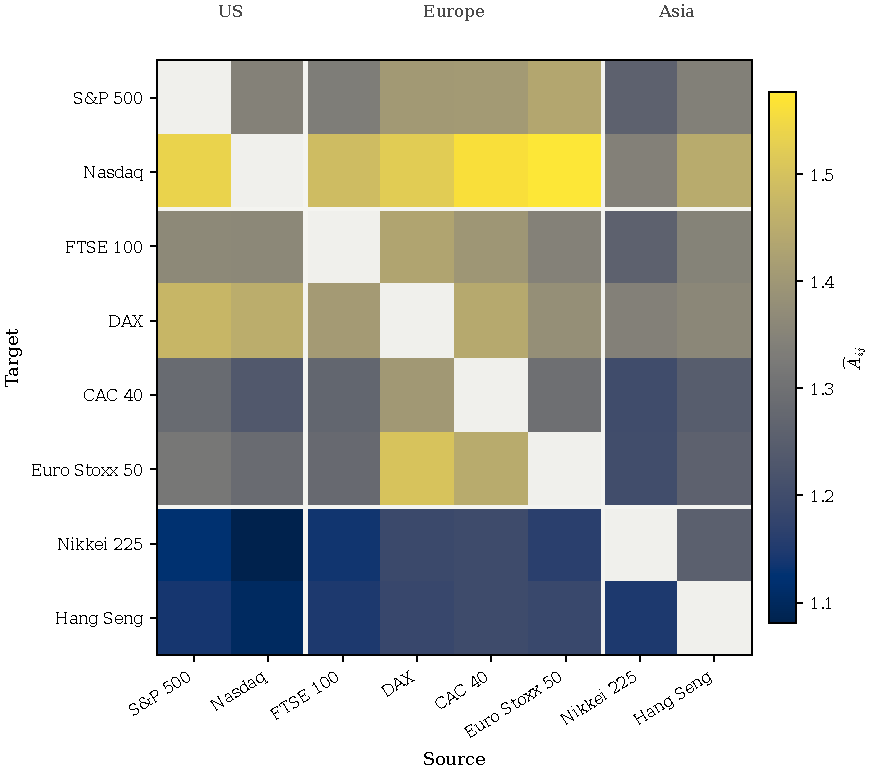
\includegraphics[width=0.82\textwidth]{figures/4-oxfordman-perron-operator.pdf}
\caption{Full-sample empirical Perron operator on the balanced eight-index Oxford-Man panel.  The
operator entries are \(\sqrt{\widehat{\mathrm{projinfo}}_{ij}}\) on directed off-diagonal edges,
with zero diagonal.}
\label{fig:perron-operator}
\end{figure}

Figure~\ref{fig:perron-operator} reports the full-sample screened operator.  The dominant eigenvalue
is separated from the subleading radius, and the Perron weights concentrate on the same cross-market
core that dominates the market-level roughness analysis.

\begin{table}[t]
\centering
\small
\begin{tabular}{ll}
\hline
Statistic & Value \\
\hline
Full-sample spectral radius $\hat\rho_1$ & 9.2354 \\
Subleading spectral radius $\hat\rho_2$ & 1.4425 \\
Concentration score $1-\hat\rho_2/\hat\rho_1$ & 0.8438 \\
Aggregate explained share $R^2$ & 0.9999 \\
Off-Perron share $S^{\mathrm{off}}$ & 0.0001 \\
Top right-load components $\hat v$ & Nasdaq (0.39), DAX (0.37), S\&P 500 (0.36) \\
Top left-load components $\hat u$ & CAC 40 (0.37), DAX (0.37), Euro Stoxx 50 (0.36) \\

\end{tabular}
\caption{Full-sample Perron summary for the Oxford-Man illustration.}
\label{tab:perron-summary}
\end{table}

Table~\ref{tab:perron-summary} reports a full-sample spectral radius of \(9.2354\) and a
concentration score of \(0.8438\).  For the aggregate reduction, the Perron-implied component
captures nearly all of the equal-weight aggregate stress proxy in this construction.  The
full-sample explained share is \(0.9999\), while the off-Perron share is \(0.0001\).  This is
consistent with the aggregate-first sufficiency claim made in Section~\ref{sec:implications}; it is
not a claim that the Perron component exhausts all latent market structure.

\begin{figure}[t]
\centering
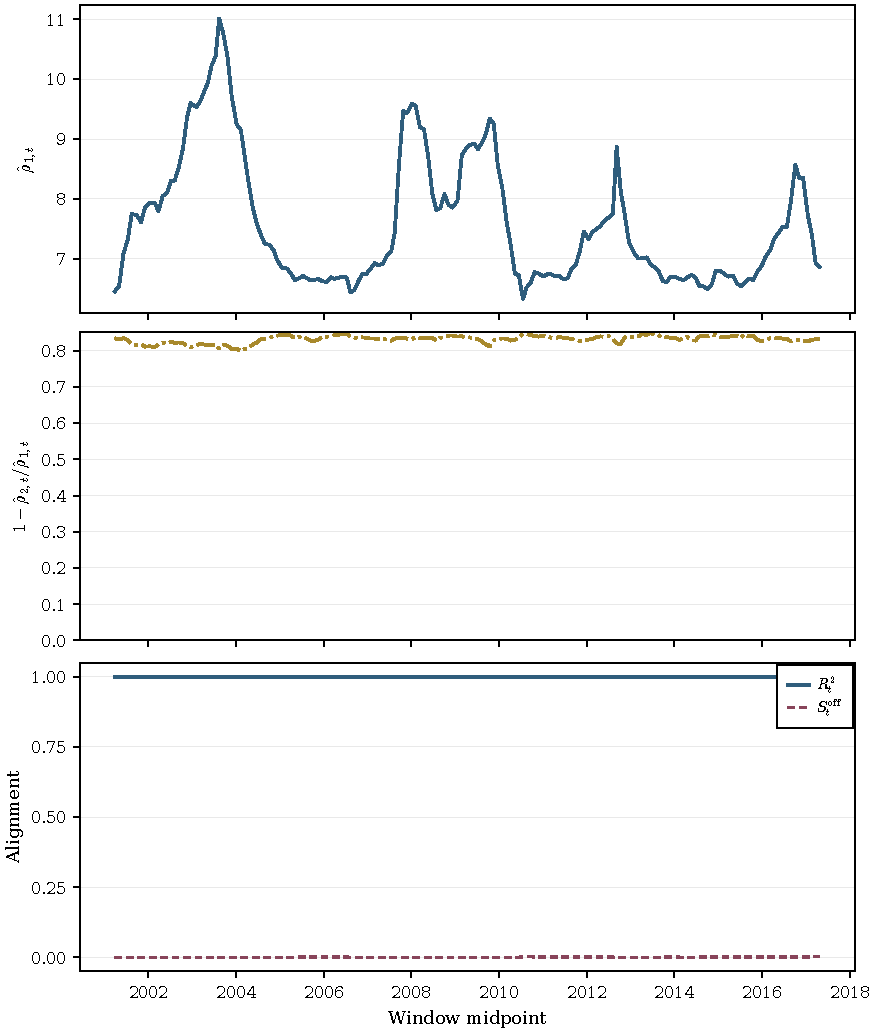
\includegraphics[width=0.88\textwidth]{figures/4-oxfordman-perron-rolling.pdf}
\caption{Rolling Perron summaries on 504-day windows stepped every 21 trading days.  The panels
show the spectral radius \(\widehat\rho_{1,t}\), the concentration score
\(1-\widehat\rho_{2,t}/\widehat\rho_{1,t}\), and the aggregate explained share \(R_t^2\) together
with the off-Perron share \(S_t^{\mathrm{off}}\).}
\label{fig:perron-rolling}
\end{figure}

Figure~\ref{fig:perron-rolling} reports rolling stability of the Perron construction.  Across the
\(171\) rolling windows, the spectral radius stays between \(6.3277\) and \(11.0111\), the
concentration score remains between \(0.7996\) and \(0.8495\), the aggregate explained share never
falls below \(0.9977\), and the off-Perron share never rises above \(0.0023\).  The aggregate
explained share remains high in both crisis and non-crisis windows.

\begin{table}[t]
\centering
\small
\begin{tabular}{lcc}
\hline
Statistic & Crisis & Non-crisis \\
\hline
Mean spectral radius $\hat\rho_1$ & 7.8085 & 7.5213 \\
Mean concentration $1-\hat\rho_2/\hat\rho_1$ & 0.8354 & 0.8308 \\
Mean aggregate explained share $R_t^2$ & 0.9994 & 0.9995 \\
Mean off-Perron share $S_t^{\mathrm{off}}$ & 0.0006 & 0.0005 \\

\end{tabular}
\caption{Rolling crisis versus non-crisis Perron summaries.}
\label{tab:perron-crisis}
\end{table}

Table~\ref{tab:perron-crisis} reports the same quantities at the regime level.  Crisis windows have
a somewhat larger mean spectral radius, but both crisis and non-crisis periods retain strong Perron
concentration and a very small aggregate off-Perron share.  The empirical statement is
quantitative.  On this realized-volatility panel, the Perron projection captures the dominant
aggregate direction while leaving only a small aggregate remainder.

\bibliographystyle{unsrt}
\bibliography{references}

\end{document}
